%%%%%%%%%%%%%%%%%%%%%%%%%%%%%%%%%%%%%%%%%%%%%%%%%%%%%%%%%%%%%%%%%%%%%%%%%%%%%%%%%%%%%%%%%%%%%%%%%%%%%%%%%%%%%%%%%%%%%%%%%%%%%%%%%%%%%%%%%%%%%%%%%%%%%%%%%%%
% This is just an example/guide for you to refer to when submitting manuscripts to Frontiers, it is not mandatory to use Frontiers .cls files nor frontiers.tex  %
% This will only generate the Manuscript, the final article will be typeset by Frontiers after acceptance.   
%                                              %
%                                                                                                                                                         %
% When submitting your files, remember to upload this *tex file, the pdf generated with it, the *bib file (if bibliography is not within the *tex) and all the figures.
%%%%%%%%%%%%%%%%%%%%%%%%%%%%%%%%%%%%%%%%%%%%%%%%%%%%%%%%%%%%%%%%%%%%%%%%%%%%%%%%%%%%%%%%%%%%%%%%%%%%%%%%%%%%%%%%%%%%%%%%%%%%%%%%%%%%%%%%%%%%%%%%%%%%%%%%%%%

%%% Version 3.4 Generated 2018/06/15 %%%
%%% You will need to have the following packages installed: datetime, fmtcount, etoolbox, fcprefix, which are normally inlcuded in WinEdt. %%%
%%% In http://www.ctan.org/ you can find the packages and how to install them, if necessary. %%%
%%%  NB logo1.jpg is required in the path in order to correctly compile front page header %%%

\documentclass[utf8]{frontiersSCNS} % for Science, Engineering and Humanities and Social Sciences articles

\usepackage{url,hyperref,lineno,microtype}
\usepackage{graphicx}
\usepackage{subcaption}
\usepackage[onehalfspacing]{setspace}
\usepackage[english]{babel}

\linenumbers

% Leave a blank line between paragraphs instead of using \\

\def\keyFont{\fontsize{8}{11}\helveticabold }
\def\firstAuthorLast{Sample {et~al.}} %use et al only if is more than 1 author
\def\Authors{First Author\,$^{1,*}$, Co-Author\,$^{2}$ and Co-Author\,$^{1,2}$}
% Affiliations should be keyed to the author's name with superscript numbers and be listed as follows: Laboratory, Institute, Department, Organization, City, State abbreviation (USA, Canada, Australia), and Country (without detailed address information such as city zip codes or street names).
% If one of the authors has a change of address, list the new address below the correspondence details using a superscript symbol and use the same symbol to indicate the author in the author list.
\def\Address{$^{1}$Laboratory X, Institute X, Department X, Organization X, City X , State XX (only USA, Canada and Australia), Country X \\
$^{2}$Laboratory X, Institute X, Department X, Organization X, City X , State XX (only USA, Canada and Australia), Country X  }
% The Corresponding Author should be marked with an asterisk
% Provide the exact contact address (this time including street name and city zip code) and email of the corresponding author
\def\corrAuthor{Corresponding Author}

\def\corrEmail{email@uni.edu}


\begin{document}
\onecolumn
\firstpage{1}

% Phenotypic plasticity can promote the evolution of complex features in fluctuating environments
% Phenotypic plasticity can simultaneously slow rate of evolutionary change and promote evo of complex features 
% Adaptive plasticity buffers population against fluctuations, promoting novel trait evolution/retention
\title[The evolutionary consequences of plasticity]{Phenotypic plasticity can promote the evolution and maintenance of complex features in fluctuating environments} 

\author[\firstAuthorLast ]{\Authors} %This field will be automatically populated
\address{} %This field will be automatically populated
\correspondance{} %This field will be automatically populated

\extraAuth{}% If there are more than 1 corresponding author, comment this line and uncomment the next one.
%\extraAuth{corresponding Author2 \\ Laboratory X2, Institute X2, Department X2, Organization X2, Street X2, City X2 , State XX2 (only USA, Canada and Australia), Zip Code2, X2 Country X2, email2@uni2.edu}


\maketitle


%%%%%%%%%%%%%%%%%%%%%%%%%%%%%%%%%%%%
% Utility commands
%%%%%%%%%%%%%%%%%%%%%%%%%%%%%%%%%%%%
\newcommand{\code}{\texttt}


%%%%%%%%%%%%%%%%%%%%%%%%%%%%%%
% Evolutionary change rate experiment
%%%%%%%%%%%%%%%%%%%%%%%%%%%%%%

% data from experiment - 2021-02-08
\newcommand{\evolutionaryChangeRateReplicates}{100}

\newcommand{\evolutionaryChangeRatePlasticReps}{42}


%%%%%%%%%%%%%%%%%%%%%%%%%%%%%%
% Novel traits experiment
%%%%%%%%%%%%%%%%%%%%%%%%%%%%%%
\newcommand{\novelTraitsReplicates}{100}
\newcommand{\novelTraitsReward}{10\%}
\newcommand{\novelTraitsPlasticReps}{42}

%%%%%%%%%%%%%%%%%%%%%%%%%%%%%%
% Deleterious hitchhiking experiment
%%%%%%%%%%%%%%%%%%%%%%%%%%%%%%
% - 2021-02-05 -
\newcommand{\deleteriousHitchhikingReplicates}{100}
\newcommand{\deleteriousHitchhikingPlasticReps}{43}
\newcommand{\instPoisonMagnitude}{10\%}

% Abstract

% Flip narrative - lead with consequence, tease apart with dynamics/controls

% Current problems: 
% - not full picture of results (not specific enough)
% - need to better place this work in context of existing work


\begin{abstract}

\section{}
Fluctuating environmental conditions are ubiquitous in natural systems, and the particular mechanisms that populations rely on to cope with environmental fluctuations profoundly influence subsequent evolutionary dynamics.
Phenotypic plasticity, the ability of a single genotype to produce alternate phenotypes, allows organisms to dynamically adjust phenotypic expression in an environmentally dependent context.
Here, we use digital organisms (self-replicating computer programs) to investigate how the evolution of adaptive phenotypic plasticity alters evolutionary dynamics and influences evolutionary outcomes in cyclically changing environments.
Specifically, we 
(1) examined the evolutionary histories of plastic and non-plastic populations to test whether the evolution of adaptive plasticity promotes or constrains subsequent evolutionary change;
(2) evaluated if adaptive plasticity improves fitness landscape exploration and exploitation by testing whether plastic populations are better able to evolve and then maintain novel traits;
% [prevalence of deleterious hitchhiking]
and (3) compared the [accumulation of deleterious genes] in plastic and non-plastic populations to test if the evolution of adaptive plasticity increases the potential for deleterious cryptic variation to accumulate.
We find that populations with adaptive phenotypic plasticity evolve more slowly than non-plastic populations, which rely on genetic variation from \textit{de novo} mutations to continuously re-adapt to the environment.
The non-plastic populations undergo more frequent selective sweeps, accumulate many more genetic changes, [finish listing big results]. 
We find that phenotypic plasticity stabilizes populations against environmental fluctuations; whereas the repeated selective sweeps in non-plastic populations drive the loss of beneficial traits via deleterious hitchhiking.  
As such, plastic populations are more likely to retain novel adaptive traits than their non-plastic counterparts. 
All natural environments subject populations to some form of change; our findings suggest that the stabilizing effect of phenotypic plasticity plays an important role in subsequent adaptive evolution.

%All article types: you may provide up to 8 keywords; at least 5 are mandatory.

\tiny
 \keyFont{ \section{Keywords:} phenotypic plasticity, evolution, digital evolution, changing environments} 

\end{abstract}

%%%%%%%%%%%%%%%%%%%%%%%%%%%%%%%%%%%%%%%%%%%%%%%%%%%%%%%%%%%%%%%%%%%%%%%%%%%%%%%%%%%%%%%%%%%%%%%%%%%%%
% The introduction should be succinct, with no subheadings. 
%%%%%%%%%%%%%%%%%%%%%%%%%%%%%%%%%%%%%%%%%%%%%%%%%%%%%%%%%%%%%%%%%%%%%%%%%%%%%%%%%%%%%%%%%%%%%%%%%%%%%

\section{Introduction}

%%%%%%%%%%%%%%%%%%%%%%
% -- Different mechanisms evolve to cope with fluctuating environments, and those mechanisms
%    affect evolution. --
%%%%%%%%%%%%%%%%%%%%%%
Fluctuating environmental conditions are ubiquitous in natural systems. 
Organisms have evolved a wide range of evolved strategies for coping with environmental change, such as 
phenotypic plasticity \citep{ghalambor_adaptive_2007}, 
bet hedging \citep{beaumont_experimental_2009}, 
periodic migration \citep{winger_long_2019}, 
and adaptive tracking \citep{barrett_adaptation_2008}.
The particular coping mechanisms that evolve in fluctuating environments shift the course of subsequent evolution \citep{wennersten_population-level_2012,schaum_plasticity_2014}.
Identifying the mechanisms most likely to evolve and examining both the evolutionary constraints and opportunities associated with each is critical for us to understand and predict evolutionary outcomes in changing environments.

%%%%%%%%%%%%%%%%%%%%%%
% -- We focus on how plasticity affects subsequent evolution. --
%%%%%%%%%%%%%%%%%%%%%%
In this work, we focus on phenotypic plasticity, which can be defined as the capacity for a single genotype to alter phenotypic expression in response to a change in its environment \citep{west-eberhard_developmental_2003}. 
Phenotypic plasticity is controlled by genes whose expression is coupled to one or more abiotic or biotic environmental signals. 
For example, the sex ratio of the crustacean \textit{Gammarus duebeni} is modulated by changes in photoperiod and temperature \citep{dunn_two_2005}, and the reproductive output of some invertebrate species is heightened when infected with parasites to compensate for offspring loss \citep{chadwick_parasite-mediated_2005}. 
In this study, we conducted digital evolution experiments to investigate how the evolution of adaptive phenotypic plasticity shifts the course of evolution in a cyclically changing environment.
Specifically, we examined the effects of adaptive plasticity on subsequent genomic and phenotypic change, the capacity to evolve and then maintain novel traits, and the accumulation of deleterious alleles.


%%%%%%%%%%%%%%
% Effects of phenotypic plasticity on subsequent evolution disputed.
%   - baseline expections on rate of evolutionary response given adaptive vs. non-adaptive plasticity
%%%%%%%%%%%%%%
Evolutionary biologists have long been interested in how evolutionary change across generations is influenced by phenotypic plasticity because of its role in generating phenotypic variance \citep{gibert_phenotypic_2019}.
The effects of phenotypic plasticity on adaptive evolution have been disputed, as few studies have been able to observe both the initial patterns of plasticity and the subsequent divergence of traits in natural populations \citep{ghalambor_adaptive_2007,wund_assessing_2012,forsman_rethinking_2015,ghalambor_non-adaptive_2015,hendry_key_2016}.
In a changing environment, adaptive phenotypic plasticity provides a mechanism for organisms to regulate trait expression within their lifetime, which can stabilize populations through changes \citep{gibert_phenotypic_2019} [conceptual figure (see comment)?].
In this context, the stabilization effects of adaptive plasticity have been hypothesized to constrain the rate of adaptive evolution \citep{gupta_study_1982,ancel_undermining_2000,huey_behavioral_2003,price_role_2003,paenke_influence_2007}.
That is, directional selection may be weak if environmentally-induced phenotypes are close to the optimum; as such, adaptively plastic populations may evolve slowly (relative to non-plastic populations) unless there is a substantial fitness cost to plasticity.

\begin{figure}[h!]
    \centering
    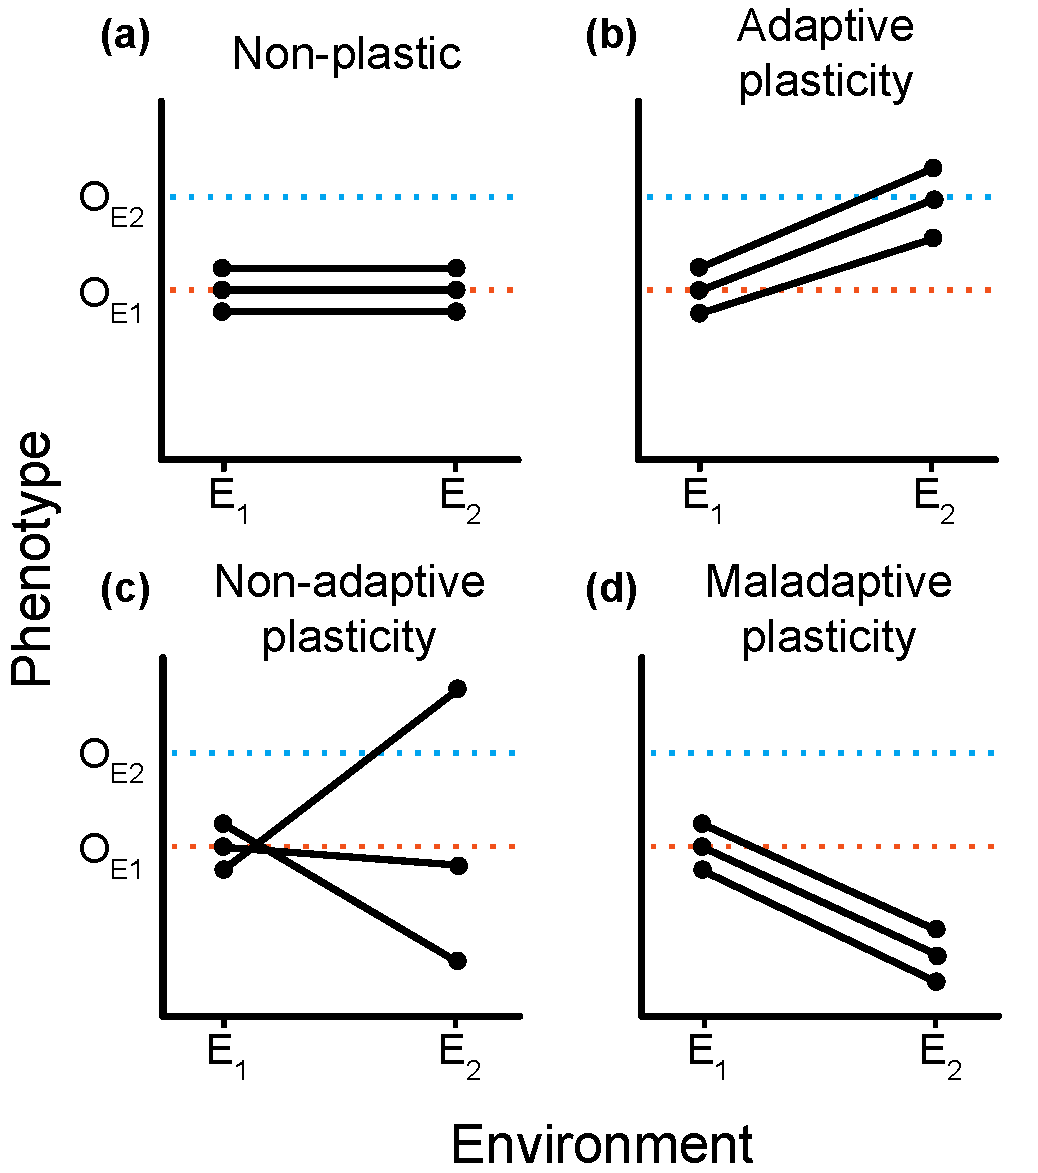
\includegraphics[width=\textwidth]{media/reaction-norms.pdf}
    \caption{\small
    \textbf{todo.}
    todo.
    }
    \label{fig:reaction-norms}
\end{figure}

% Feedback
%  - Ideas: color background red/blue
%  - Titles on (a), (b), (c), (d)?
%    - Swap (c) & (d)
%    - non-plastic, adaptive plasticity, non-adaptive plasticity, maladaptive plasticity
%  - (e) environmental scenario/environment
% - Increase font sizes
% - pull word that says time outside the arrow, make arrow smaller, make environment bar bigger => increase font size

% -- Plasticity as a source of cryptic variation --
Phenotypic plasticity allows for the accumulation of genetic variation in genomic regions that are unexpressed under current environmental conditions.
Such cryptic (``hidden'') genetic variation can serve as a source of diversity in the population, upon which selection can act when the environment changes \citep{schlichting_hidden_2008,levis_evaluating_2016}.  
It remains unclear to what extent and under what circumstances this cryptic variation caches adaptive potential or merely accumulates deleterious alleles \citep{gibson_uncovering_2004,paaby_cryptic_2014,zheng_cryptic_2019}.

% -- Genes as followers --
The ``genes as followers'' hypothesis (also known as the ``plasticity first'' hypothesis) predicts that phenotypic plasticity may facilitate adaptive evolutionary change by producing variants with enhanced fitness under stressful or novel conditions \citep{west-eberhard_developmental_2003,schwander_genes_2011,levis_evaluating_2016}. 
Environmentally-induced trait changes can be refined through selection over time (i.e., genetic accommodation).
Further, selection may drive plastic phenotypes to lose their environmental dependence over time in a process known as genetic assimilation \citep{west-eberhard_developmental_2005,pigliucci_phenotypic_2006,crispo_baldwin_2007,schlichting_phenotypic_2014,levis_evaluating_2016}. 
In this way, environmentally-induced phenotypic changes can precede an evolutionary response.

% -- Plastic rescue + wrap up on plasticity background? --
Phenotypic plasticity may also `rescue' populations from extinction under changing environmental conditions by buffering populations against novel stressors.
This buffer promotes stability and persistence and grants populations time to further adapt to rapidly changing environmental conditions \citep{west-eberhard_developmental_2003,chevin_when_2010}. %[citations - Snell-Rood et al. 2018?].
Disparate predictions about how phenotypic plasticity may shift the course of subsequent evolution are not necessarily mutually exclusive.
Genetic and environmental contexts determine if and to what extent phenotypic plasticity promotes or constrains subsequent evolution.

%%%%%%%%%%%%%%%%%%%%%%
% -- Digital evolution --
%%%%%%%%%%%%%%%%%%%%%%
Experimental studies investigating the relationship between phenotypic plasticity and evolutionary outcomes can be challenging to conduct in natural systems.
Such experiments would require the ability to irreversibly toggle plasticity followed by long periods of evolution during which detailed phenotypic data would need to be collected.
Digital evolution experiments have emerged as a powerful research framework from which evolution can be studied.
In digital evolution, self-replicating computer programs (digital organisms) compete for resources, mutate, and evolve following Darwinian dynamics  \citep{mckinley_harnessing_2008}.
Digital evolution studies balance the speed and transparency of mathematical and computational simulations with the open-ended realism of laboratory experiments.
Modern computers allow us to observe many generations of digital evolution at tractable time scales; thousands of generations can take mere minutes as opposed to months, years, or centuries.
Digital evolution systems also allow for perfect, non-invasive data tracking.
Such transparency permits the tracking of complete evolutionary histories within an experiment, which circumvents the historical problem of drawing evolutionary inferences using incomplete records (from frozen samples or even fossils) and extant genetic sequences.
Additionally, digital evolution systems allow for experimental manipulations and analyses that go beyond what is possible in wet-lab experiments.
Such analyses have included exhaustive knockouts of every loci to identify the functionality of each \citep{lenski_evolutionary_2003},
comprehensive characterization of local mutational landscapes \citep{lenski_genome_1999,canino-koning_fluctuating_2019},
and the real-time reversion of all deleterious mutations as they occur to isolate their long-term effects on evolutionary outcomes \citep{covert_experiments_2013}. 
Digital evolution studies allow us to directly toggle the possibility for adaptive plastic responses to evolve, which enables us to empirically test hypotheses that were previously relegated to theoretical analyses.

%%%%%%%%%%%%%%%%%%%%%%
% -- Overview of what we're testing / doing --
%%%%%%%%%%%%%%%%%%%%%%
In this work, we use the Avida Digital Evolution Platform \citep{ofria_avida:_2009}.
Avida is an open-source system that has been used to conduct a wide range of well-regarded studies on evolutionary dynamics, including 
the origins of complex features \citep{lenski_evolutionary_2003},
the survival of the flattest effect \citep{wilke_evolution_2001},
and the origins of reproductive division of labor \citep{goldsby_evolutionary_2014}.
% @AML: next bit is a little awkward
Our experiments build directly on previous studies in Avida that characterized the \textit{de novo} evolution of adaptive phenotypic plasticity \citep{clune_investigating_2007,lalejini_evolutionary_2016} and studies that characterized the evolutionary consequences of fluctuating environments for populations of non-plastic digital organisms \citep{wilke_evolution_2001,canino-koning_fluctuating_2019}.
Of particular relevance, \cite{clune_investigating_2007} and \cite{lalejini_evolutionary_2016} experimentally demonstrated that adaptive phenotypic plasticity can evolve given the following four conditions (as identified by \cite{ghalambor_behavior_2010}):
(1) populations experience temporal environmental variation,
(2) these environments are differentiable by reliable cues,
(3) each environment favors different phenotypic traits,
and (4) no single phenotype exhibits high fitness across all environments.
% \cite{wilke_evolution_2001}....
% \cite{canino-koning_evolution_2016}....
We build on this previous work but shift our focus from the evolutionary causes of adaptive phenotypic plasticity to investigate its evolutionary consequences in a fluctuating environment.

% Here, we empirically investigate how adaptive phenotypic plasticity affects subsequent evolutionary dynamics in a fluctuating environment.
%%%%%%%%%%%%%%%%%

% - what we did -
Each of our experiments are divided into two phases: in phase one, we precondition sets of founder organisms with differing plastic or non-plastic adaptations;
in phase two, we examine the subsequent evolution of populations founded with organisms from phase one under specific environmental conditions [figure].
First, we examine the evolutionary histories of phase two populations to test whether adaptive plasticity constrained subsequent genomic and phenotypic changes. 
Next, we evaluate how adaptive plasticity influences fitness landscape exploration and exploitation by identifying how well populations produced by each type of founder are able to evolve and retain novel adaptive traits.
Finally, we test whether adaptive plasticity facilitated the accumulation of deleterious genes via cryptic genetic variation by measuring the frequency with which deleterious mutations occur along successful lineages. 
% [Finally we examine the frequency with which deleterious mutations occur along successful lineages in each type of population in order to understand how and why different types of plasticity allow or prevent].

%%%%%%%%%%%%%%%%%%%%%%
% - Overview of findings -
%%%%%%%%%%%%%%%%%%%%%%
% TODO - incorporate architecture results
We found that the evolution of adaptive plasticity reduced subsequent rates of evolutionary change in a cyclic environment.
% We found that adaptively plastic populations evolve more slowly than non-plastic populations in a cyclic environment. 
The non-plastic populations underwent more frequent selective sweeps and accumulated many more genetic changes over time, as non-plastic populations relied on genetic variation from \textit{de novo} mutations to continuously re-adapt to environmental changes. 
We found that the evolution of adaptive phenotypic plasticity buffers populations against environmental fluctuations, whereas repeated selective sweeps in non-plastic populations drive the accumulation of deleterious genes and the loss of secondary beneficial traits via deleterious hitchhiking.
As such, adaptively plastic populations were better able to retain novel traits than their non-plastic counterparts.
% In addition, we did not find evidence that the evolution of adaptive plasticity resulted in increased rates of deleterious mutation accumulation. 


% Our results suggest that adaptive phenotypic plasticity can improve the potential for populations exploit novel resources in cyclically changing environments.

%%%%%%%%%%%%%%%%%%%%%%%%%%%%%%%%%%%%%%%%%%%%%%%%%%%%%%%%%%%%%%%
% JOURNAL INSTRUCTIONS
% This section may be divided by subheadings and should contain sufficient detail so that when read in conjunction with cited references, all procedures can be repeated. For experiments reporting results on animal or human subject research, an ethics approval statement should be included in this section (for further information, see the Bioethics section.)
%%%%%%%%%%%%%%%%%%%%%%%%%%%%%%%%%%%%%%%%%%%%%%%%%%%%%%%%%%%%%%%

%%%%%%%%%%%%%%%%%%%%%%%%%%%%%%%%%
% Questions for 2021-03-09
% - How should we structure: Experimental Design => Results => Discussion
%   - We conducted 3 separate experiments. Currently, we discuss each experiment separately across sections. (1) do we want to stick to this structure? (2) if so, what should the headings be?
% - What parts of what is currently experimental design belong in methods vs. results. vs discussion?
%   - I 100% want to provide some intuition about measurements (in the paper), but where? I'd like trainees to be able to read this as easily as possible. 
% - I do actually think the details for the metrics/measurements are important. 
% - Discuss the overall flow of the methods section. Should the 'quantifying tape of life' metrics actually be under experiment 1 since that's what they are relevant to?
% - I think we could combine results and discussion? Other major re-organizations?
% - 'mutation accumulation'
%%%%%%%%%%%%%%%%%%%%%%%%%%%%%%%%%

\section{Materials and Methods}

% -- bookmark --

\subsection{The Avida Digital Evolution Platform}

% We conducted our study using the Avida Digital Evolution Platform \citep{ofria_avida:_2009}. 
% Avida provides a computational study system where populations of digital organisms undergo Darwinian evolution, allowing researchers to test hypotheses that would be difficult or impossible to address in natural systems.

% - Define digital organisms -
Avida is a study system wherein self-replicating computer programs (digital organisms) compete for space on a finite toroidal grid \citep{ofria_avida:_2009}.
Each digital organism is defined by a linear sequence of program instructions (its genome) and a set of virtual hardware components used to interpret and express those instructions. 
% Avida tracks each organism as it expresses its genome in a given environment in order to measure that organism's phenotype.
Genomes are expressed sequentially except when the execution of one instruction deterministically changes which instruction should be executed next (e.g., a `jump' instruction). 
Genomes are built using an instruction set that is both robust (\textit{i.e.}, any ordering of instructions is syntactically valid, though not necessarily meaningful) and Turing Complete (\textit{i.e.}, able to represent any computable function, though not necessarily in an efficient manner) [cite].
% ; that is, any ordering of instructions is syntactically valid (though not necessarily meaningful), and genomes are able to represent any computable function (though not necessarily in an efficient manner).
The instruction set includes operations for basic computations, flow control (e.g., conditional logic and looping), input, output, and self-replication.
% @AML: Outsource the next sentence to a figure!
% The virtual hardware set includes components such as a central processing unit (CPU) for executing instructions, registers to store values, buffers for inputs and outputs, and memory stacks \citep{ofria_avida:_2009}.

% \begin{figure}[h!]
    \centering
    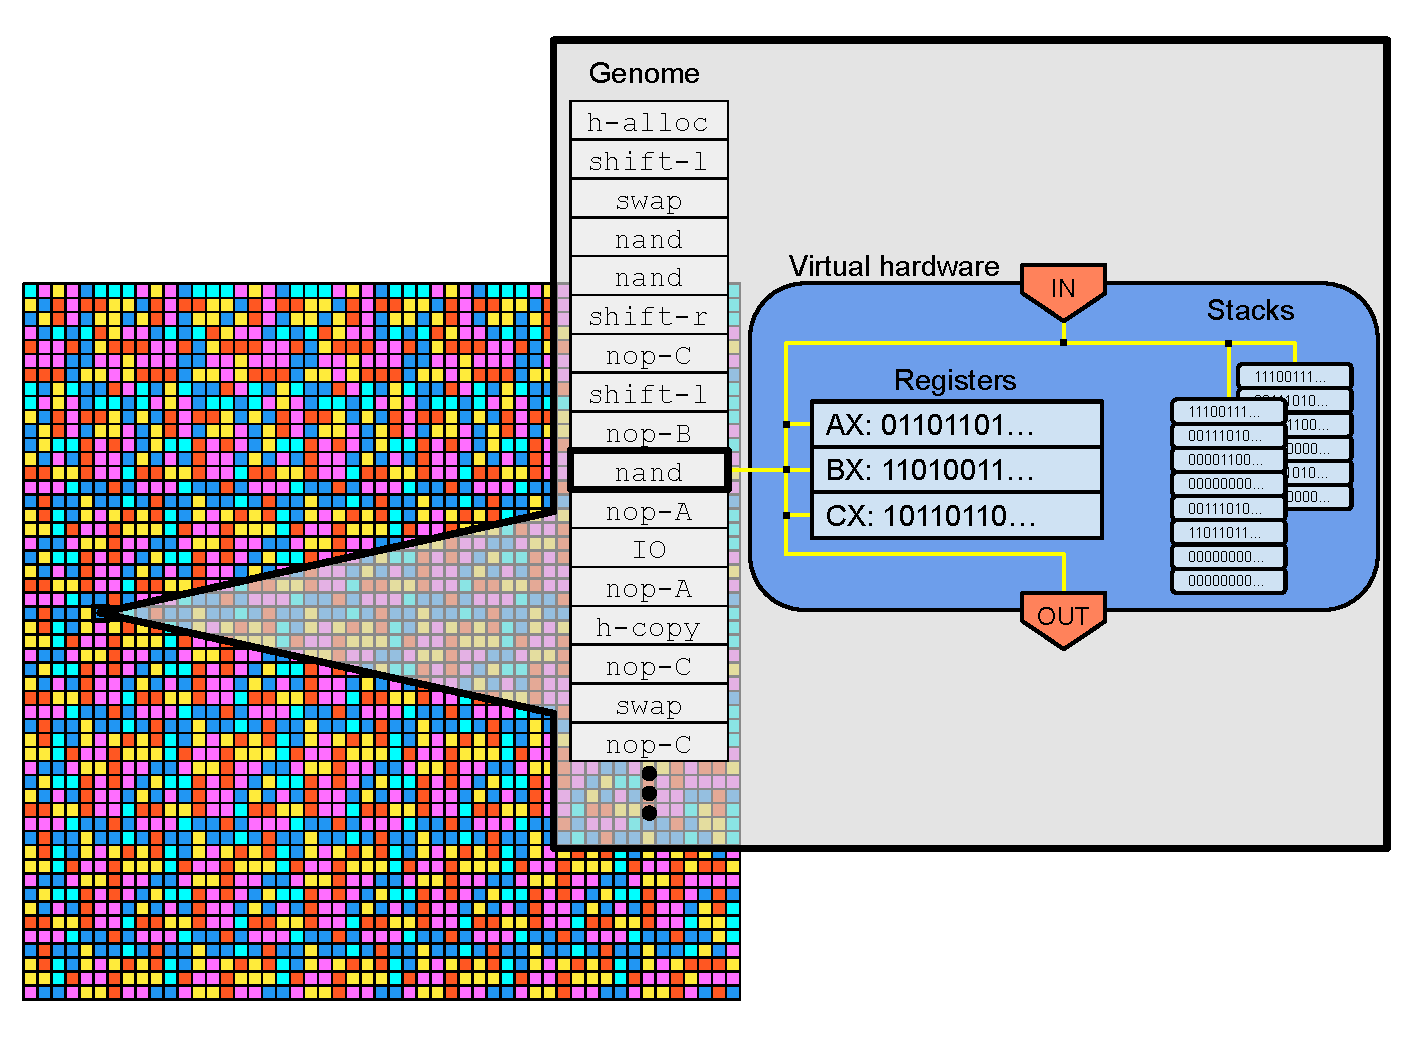
\includegraphics[width=\textwidth]{media/avida-hardware.pdf}
    \caption{\small
    \textbf{todo.}
    todo.
    }
    \label{fig:avida-virtual-hardware}
\end{figure}

% Feedback:
%  - make grid non-repetitive
%    - as tile rotate
%  - output a task? 
%    - one of first 6


% - define reproduction & mutation -
Organisms in Avida reproduce asexually by copying their genome instruction-by-instruction and then dividing. 
However, copy operations are imperfect and can result in single-instruction substitution mutations in an offspring's genome. 
For this work, we configured copy operations to err at a rate of one expected mutation for every 400 instructions copied (i.e, a per-instruction error rate of 0.0025).
% at a per-instruction rate of 0.0025 (i.e., one mutation expected for every 400 instructions copied).
We held individual genomes at a fixed length of 100 instructions; that is, we did not include insertion and deletion mutations. 
We used fixed-length genomes to control for treatment-specific conditions resulting in the evolution of substantially different genome sizes [supplement, citations]\footnote{We repeated our experiments without genome size restrictions and observed qualitatively similar results [cite supplement].}, which could, on its own, drive differences in evolutionary outcomes among experimental treatments.
When an organism divides in Avida, its offspring is placed in a random location on the toroidal grid, replacing any previous occupant.
For this work, we used the default 60 by 60 grid size, which limits the maximum population size to 3600 organisms.
As such, improvements to the speed of self-replication are advantageous in the competition for space.
% The combination of this competition for space and heritable variation from imperfect replication results in evolution by natural selection.

% Avida tracks each organism as it expresses its genome in a given environment in order to measure that organism's phenotype.

% - define fitness/metabolic rate/improving replication speed -
During evolution, organism replication rates improve in two ways: by improving genome efficiency (e.g., using a more compact encoding) or by accelerating the rate at which the genome is expressed (their ``metabolic rate'').
An organism's metabolic rate determines the speed at which it executes instructions in its genome.
Initially, an organism's metabolic rate is proportional to the length of its genome, but that rate is adjusted as it completes designated tasks, such as performing Boolean logic computations \citep{ofria_avida:_2009}.
In this way, we can reward or punish particular phenotypic traits. 

\subsubsection{Phenotypic plasticity in Avida}

%%%% TODO - EDIT THIS SECTION

% -- Phenotypes & Phenotypic plasticity --
% - What is a phenotype in Avida
In this work, we measure a digital organism's phenotype as the set of Boolean logic functions that it performs in a given environment.
Sensory instructions in the Avida instruction set allow organisms to detect how performing a particular logic function would affect their metabolic rate [cite - supplement]. 
We define a phenotypically plastic organism as one that uses sensory information to alter which logic functions it performs based on the environment.

% -- Adaptive plasticity & non-adaptive plasticity --
Phenotypic plasticity in Avida can be adaptive or non-adaptive for a given set of environments.
Adaptive plasticity shifts net task expression closer to the optimum for the given environments.
% Non-adaptive plasticity either changes task expression in a neutral way or further from the optimum for a given set of environments.
Non-adaptive plasticity changes task expression in either a neutral or deleterious way.% for a given set of environments.
Optimal plasticity changes tasks to always perfectly match the set of rewarded tasks.% for each environment.

% For the majority of our experiments, we focus on the following 6 one- and two-input logic functions: NOT, NAND, AND, OR-NOT, OR, and AND-NOT. 
% An organism's \textit{comprehensive} or \textit{aggregate} phenotype is characterized by the set of logic functions performed in each of a set of given environments. 

% \vspace{1cm}
% \subsubsection{Evolving adaptive phenotypic plasticity in Avida}
% \label{sec:methods:evolution-of-plasticity-in-avida}

% @AML: Based on Nkrumah's feedback, I think this section needs to be reorganized. 
\vspace{0.7cm}
\subsection{Experimental design}
\label{sec:methods:experiment}

%%%%%%%%%%%%%%%%%%%%%%%%%%%%%%%%%%%%%%%%%%%%%%%%%
% OUTLINE
%%%%%%%%%%%%%%%%%%%%%%%%%%%%%%%%%%%%%%%%%%%%%%%%%
% Overview of experimental design - with diagram (not a subsubsection?)
% - Focused around diagram
% Environment implementations
% Specifications for Phase 1
% specifications for Phase 2A
% specifications for Phase 2B
% specifications for Phase 2C
% Measurements and Analyses
% - number of coalescence
% - mutation accumulation
% - phenotypic volatility
% - mutational stability
% - genetic architectures
% - novel task performance
% - novel task discovery
%%%%%%%%%%%%%%%%%%%%%%%%%%%%%%%%%%%%%%%%%%%%%%%%%

% -- Overview of experimental design --
We conducted three independent experiments using Avida to investigate how the evolution of adaptive plasticity influences evolutionary outcomes in fluctuating environments.
% @AML: 1 liner of what each of these experiments were? IDK, this info is in the intro, so maybe not important here.
For each experiment, we compared the evolutionary outcomes of populations evolved under three treatments (Figure [XX]): 
(1) a \textbf{PLASTIC} treatment where the environment fluctuates, and digital organisms can use sensory instructions to differentiate between environmental states;
(2) a \textbf{NON-PLASTIC} treatment with identical environment fluctuations, but where sensory instructions are disabled;
and (3) a \textbf{STATIC} control where organisms evolve in a constant environment.

% @AML: maybe cut this next sentence
% These experiments build directly on previous digital evolution studies on the evolution of adaptive phenotypic plasticity \citep{clune_investigating_2007,lalejini_evolutionary_2016} and on the evolutionary consequences of fluctuating environments \citep{wilke_evolution_2001,canino-koning_fluctuating_2019}.
Each experiment was divided into two phases that each lasted for 200,000 updates \footnote{
    One update in Avida is the amount of time required for the average organism to execute 30 instructions. 
    See \citep{ofria_avida:_2009} for more details.
} of evolution (Figure [XX]), which is approximately 30,000 to 40,000 generations.
In phase one of each experiment, we preconditioned populations to their treatment-specific conditions.
% Each experiment shares a common setup for phase one (described in Section \ref{sec:methods:experiment:phase-one}). 
In phase two, we founded new populations with the evolved organisms from phase one and examined their subsequent evolution under given combinations of treatment and experimental conditions.
%In phase two, we examined the subsequent evolution of populations founded with organisms from phase one under given treatment conditions.
% Phase two differed among each of our experiments (described in Sections [X,Y,and Z]). %, depending the goal of the particular experiment.]
During phase two, we tracked each population's evolutionary history as well as saving the full final population.
% , and all comparisons between treatments were performed on these data.
Phase one was for pre-conditioning only; all comparisons between treatments were performed on phase two data. % from populations during phase two.

% -- Phase one => Phase two --
% @AML: I could see these details moving to their respective 'phase sections'!!
% At the beginning of phase one [in each experiment], we founded 100 independent [replicate?] populations for each of three treatment conditions (described below).
% Each phase-one population was founded with a common ancestral strain capable only of self-replication [cite - supplement].
% At the end of phase one, we used the most abundant genotype from each replicate to found a new population for phase two. 
% During phase two, we evolved these new populations in their treatment-specific conditions, tracking their evolutionary history as well as saving the full final population.
% All comparisons between treatments were performed on data from populations during phase two.

\subsubsection{Environments}
\label{sec:methods:experiment:environments}

% ----- ENVIRONMENTS -----
% traits_set_a <- c("not", "and", "or")
% traits_set_b <- c("nand", "ornot", "andnot")

% -- Environment definitions --
We constructed three experimental environments, abbreviated hereafter as ``ENV-A'', ``ENV-B'', and ``ENV-ALL'' ([Figure XX]).
%Six Boolean logic tasks (...) are each rewarded or punished in each environment, as described in Figure YY.
Figure YY describes these environments based on whether each of six Boolean logic tasks (...) is rewarded or punished.
% Each rewarded task performed by an organism doubles their metabolic rate (allowing them to execute twice as many instructions in the same amount of time), and each punished task performed halves their metabolic rate. 
% A task performed by an organism doubles their metabolic rate if it is rewarded (allowing them to execute twice as many instructions in the same amount of time), or halves their metabolic rate if it is punished. 
A rewarded task performed by an organism doubles their metabolic rate, allowing them to execute twice as many instructions in the same amount of time.
A punished task halves an organisms metabolic rate. 


% --- TODO - Move these descriptions to the figure caption ---
% In ENV-A, organisms are rewarded for performing NOT, AND, and OR, but are punished for performing the NAND, OR-NOT, and AND-NOT logic tasks.
% Conversely in ENV-B, organisms are rewarded for performing NAND, OR-NOT, and AND-NOT, but are punished for performing NOT, AND, and OR. 
% Finally, in ENV-ALL, all six tasks are rewarded and none are punished.
% ------------------------------------------------

% @AML: Add deleted text to figure caption.
% Organisms with phenotypes that align with their current environment will quickly outcompete those with mismatched phenotypes.  
% A perfect match in ENV-A or ENV-B will have a metabolic bonus of $\times{8}$, a perfect mismatch will have a penalty of $\times{0.125}$, and an organism that does no tasks or all tasks will not have a modifier at all. 

% -- Treatment-specific environment details --
In both the PLASTIC and NON-PLASTIC conditions, the environment cycles between equal-length periods of ENV-A and ENV-B.
Each of these periods persist for 100 updates (approximately 15 to 20 generations).
Thus, populations experience a total of 1,000 full periods of ENV-A interlaced with 1,000 full periods of ENV-B during each experimental phase.

% -- Sensory instructions + control flow and controlling the capacity for plasticity --
% @AML: Not description of an environment, but it is how organisms sense the environment. Not sure where else this would go.
Organisms in the PLASTIC treatments differentiate between ENV-A and ENV-B by executing one of six sensory instructions, each associated with a particular logical task; these sensory instructions detect whether their associated task is currently rewarded or punished (see Supplemental Section [blah] for details [cite]).
By using sensory information in combination with execution flow-control instructions, organisms can conditionally perform different logic tasks depending on the current environmental conditions.

\subsubsection{Experiment Phase 1 -- Environment preconditioning}
\label{sec:methods:experiment:phase-one}
% @AML: if we use 'phase 1' and 'phase 2X' in headings, should we switch all 'phase one' text to 'phase 1' etc?

For each treatment, we founded 100 independent populations from a common ancestral strain capable only of self-replication [cite - supplement].
% Each phase-one population was founded with a common ancestral strain capable only of self-replication [cite - supplement].
%Phase one gives populations time (200,000 updates) to adapt to their treatment conditions, affording adaptive phenotypic plasticity the opportunity to evolve \textit{de novo} in the PLASTIC treatment.
At the end of phase one, we extracted the most abundant (i.e., dominant) genotype from each replicate population to found a new population for phase two.

%The evolution of adaptive phenotypic plasticity is not a guaranteed outcome in phase one of the PLASTIC treatment.
For the PLASTIC treatment, we measure plasticity by independently testing a given genotype in each of ENV-A and ENV-B.
We discard phase one populations if the dominant genotype does not exhibit optimal plasticity.
% @AML: not sure this is the *best* way to define optimal plasticity (it misses on it being okay if the genome performs neutral tasks).
% An optimally plastic genotype expresses only the NOT, AND, and OR logic functions in ENV-A and performs only the OR-NOT, OR, and AND-NOT in ENV-B.
% An optimally plastic genotype expresses each of the rewarded tasks in a given environment and none of the punished tasks in that environment.
This approach ensures that measurements taken on PLASTIC-treatment populations during the second phase of each experiment reflect the evolutionary consequences of adaptive plasticity.
%are representative of populations with adaptive phenotypic plasticity.

% We consider a genotype to be plastic if it expresses a different set of tasks when [tested/cultured] in ENV-A than when [tested] in ENV-B.
% Genotypes labeled \textit{optimally} plastic express each of the rewarded tasks in a given environment and none of the punished tasks in that environment.

% ---bookmark---

\subsubsection{Experiment Phase 2A -- Evolutionary change rate}
% Testing evolutionary change

% To test whether the evolution of adaptive plasticity
% constrains the rate of subsequent evolutionary change, we 
% [1 sentence of motivation/hypothesis?].
Phase two continued exactly as phase one, except we tracked the rates of evolutionary change in each of the PLASTIC-, NON-PLASTIC-, and STATIC-treatment populations. 
Specifically, we quantified evolutionary change rates using four metrics (defined in Section [X]):
(1) number of coalescence events,
(2) mutation accumulation, 
(3) phenotypic volatility,
and (4) mutational stability.
We additionally examined how the genetic architectures of organisms and their ancestors changed over time.  

\subsubsection{Experiment Phase 2B -- Novel task evolution}

% [1 sentence of motivation/hypothesis?].
Phase two continued exactly as phase one, except we used the expanded task set of 77 Boolean logic tasks during the second phase of evolution \citep{ofria_avida:_2009}.
This task set includes the six phase one tasks (NOT, NAND, AND, OR-NOT, OR, and AND-NOT; hereafter called ``base'' tasks) plus 71 new phase two tasks (hereafter called ``novel'' tasks).
Under all experimental treatments, organisms could improve their metabolic rate by performing any of the 71 novel tasks.
The six base tasks were still present in the environment and continued to be rewarded or punished according to the particular treatment conditions.
% @AML: line below is cut-able if necessary
As such, in fluctuating environments, the six base tasks continued to fluctuate, but the additional 71 tasks were always rewarded; in static environments, performing any of the 77 logic tasks was always beneficial.
% @AML: not sure where this next sentence belongs
During this experiment, we tracked the extent to which populations evolving under each treatment were capable of acquiring and retaining novel tasks.  

An organism received a \novelTraitsReward\ metabolic rate improvement for each of the novel tasks it performed (limited to one reward per unique task).
This reward provided a selective pressure to evolve these tasks, but their benefits did not overwhelm existing treatment-specific selective pressures.
As such, populations in the PLASTIC and NON-PLASTIC treatments could not easily escape environmental fluctuations by abandoning the fluctuating base tasks.

\subsubsection{Experiment Phase 2C -- Deleterious instruction accumulation}

% [In this experiment,] we tested the propensity for deleterious instructions to accumulate in genomes under each of the PLASTIC, NON-PLASTIC, and STATIC treatments.
Phase two continued exactly as phase one, except we added a \code{poison} instruction to the instruction set during phase two.
When executed by an organism, the \code{poison} instruction reduces the organism's metabolic rate (and thus reproductive success), but does not otherwise alter the organism's function.
We imposed a 10\% penalty each time an organism executed the \code{poison} instruction, making the instruct explicitly deleterious (see [supplementary material] for tests with 3\% and 30\% penalties, which produced consistent experimental results).
% @AML: want a sentence about what we tracked?
[We measured/tracked the number of times a \code{poison} instruction is executed by each genotype along the dominant lineage (including the final dominant genotype).]

% - measurements -
% @AML: This could get moved to the results?
% At the beginning of phase two, the \code{poison} instruction is not present in the population as it was not part of the instruction set during the first phase of evolution.
% However, by adding \code{poison} to the instruction set during phase two, it can be introduced via a mutation.
% We measured deleterious mutation accumulation by examining the number of times a \code{poison} instruction is executed by each genotype along the dominant lineage (including the final dominant genotype).
% Because the \code{poison} instruction is explicitly deleterious, selection should purge mutations that increase \code{poison} execution in the offspring phenotype.
% As such, we expected such mutations to show up in successful lineages either as accumulated cryptic variation in plastic genomes or via hitchhiking with linked beneficial mutations [cite].

\subsubsection{Measurements and experimental analyses}

% Evolutionary history

% Lineages and phylogenies
% - number of coalescence
% - mutation accumulation
% - phenotypic volatility
% - mutational stability
% - novel task performance
% - novel task discovery
% - genetic architectures

% - How we extracted representative lineages -
For each of our experiments, we tracked and analyzed the phylogenetic histories of evolving populations during phase two. 
For each replicate, we isolated a representative lineage from its founding organism to a member of the dominant (i.e., most abundant) genotype at the end of its evolution.
Because our experimental treatments do not support long-term coexistence, each of these lineages represented the majority of evolutionary history from a given population at the end of our experiment.

% - Measuring evolutionary change -
We quantified rates of evolutionary change using the following four metrics:
(1) number of \textbf{coalescence events} that have occurred, which indicates the frequency of selective sweeps in the population;
(2) \textbf{mutation accumulation}, which is the sum of all mutations that have occurred along a lineage;
(3) \textbf{phenotypic volatility}, which is the number of instances where parent and offspring phenotypes do not match along a lineage, as measured under a given condition;
and (4) \textbf{mutational stability}, which is the proportion of \textit{mutated} offspring along a lineage whose phenotypes do not match that of their parent, as measured under a given condition.

% - Methods for computing volatility -
To calculate phenotypic volatility for a given lineage, we expressed (i.e., evaluated) each genotype along that lineage in a treatment-specific condition, and we summed the number of changes in task profiles between consecutive genotypes.
For lineages evolved in environments fluctuating between ENV-A and ENV-B, we evaluate genotypes in both environmental conditions and count only changes in its \textit{aggregate} phenotype; this technique ensures that environmentally-induced changes are excluded from our measurement.
Phenotypic volatility as defined here illuminates the rate at which accumulated genetic changes actually change the phenotype along a lineage.

% - Methods for computing mutational stability
We measured mutational stability as the fraction of mutated offspring along a given lineage with a different phenotype than their parent.
For lineages evolved in fluctuating environments, we evaluated mutants under both ENV-A and ENV-B and counted all changes in the \textit{aggregate} task profile; like our measure of phenotypic volatility, this technique ensures that environmentally-induced changes are excluded from our measurement.
Mutational stability examines the frequency at which mutations effect changes in an offspring's phenotype.
 
In experiments that introduce novel tasks during phase two, we measured task discovery, task performance, and task loss along representative lineages.
\textbf{Task discovery} measures a given lineage's level of \textit{exploration} of the fitness landscape (i.e., the mapping between genetic space and phenotype space) \citep{canino-koning_fluctuating_2019}. 
We calculated task discovery as the total number of unique tasks ever performed along the lineage, even if a task is later lost; as such, a lineage's task discovery measurement ranged from 0 to 71.

\textbf{Task performance} measures the level of \textit{exploitation} of the fitness landscape at a given point in time.
In this work, we summarized task performance using a count of unique tasks completed by a representative organism from each population.
We focused on an organism from the dominant genotype at the end of the experiment as the most representative phenotype in the evolved population.

\textbf{Task loss} measures how often a lineage fails to retain evolved traits over time and thus indicates the ability for traits to be maintained over time.
We calculated task loss as the number of times along a lineage that a task is performed by a parent but not its offspring. 

% \subsubsubsection{Genetic architectures}

% While Avida clearly defines the mechanics of each instruction, the emergent function of an instruction depends on its context within a genome. 

% @AML: this is a little jarring
For an individual organism, we can perform \textbf{knockout experiments} to identify which instructions are responsible for producing a given phenotypic outcome.
To perform a knockout, we duplicate the organism, replacing a single instruction with an inert ``no-operation'' instruction.
We then identify any phenotypic changes by contrasting the execution results of the ``knockout'' organism and the original.
Such changes provide evidence of the role that the original instruction must have played in the genome.
For example, when an organism performs the NAND task but loses it when an instruction is knocked out, we categorize that instruction as part of the NAND task machinery.
% @AML: maybe move next sentence to results?
We use knockout experiments to characterize the role of each instruction in the genomes of every organism along all study lineages, revealing how genetic architectures change over time.

\vspace{0.5cm}
\subsection{Statistical analyses and software availability}

Across all of our experiments, we differentiated between sample distributions using non-parametric statistical tests.
For each major analysis, we first performed a Kruskal-Wallis test \citep{kruskal_use_1952} to 
determine if there were significant differences in results from the PLASTIC, NON-PLASTIC, and STATIC treatments.
If so, we applied a Wilcoxon rank-sum test \citep{kotz_individual_1992} to distinguish between pairs of treatments.
We applied Bonferroni corrections for multiple comparisons \citep{rice_analyzing_1989} where appropriate.

We conducted our experiments using a modified version of the Avida software, which is open source and freely available on GitHub [cite].
We used Python [cite] for data processing, and we conducted all statistical analyses using R version [x] [cite].
We used the tidyverse collection of R packages [cite] to wrangle data, and we used the following R packages for graphing and visualization: [list and citations].
We used R markdown [cite] and bookdown [cite] to generate web-enabled supplemental material.
All of the source code for our experiments and analyses, including guides for replication and configuration files, can be found in our supplemental material [cite].
Additionally, our experimental data is available on the Open Science framework at [url] [cite].

%%%%%%%%%%%%%%%%%%%%%%%%%%%%%%%%%%%%%%%%%%%%%%%%%%%%%%%%%%%%
% INSTRUCTIONS:
% This section may be divided by subheadings. Footnotes should not be used and must be transferred to the main text.
%%%%%%%%%%%%%%%%%%%%%%%%%%%%%%%%%%%%%%%%%%%%%%%%%%%%%%%%%%%%

\section{Results}

\subsection{Adaptive phenotypic plasticity slows evolutionary change in fluctuating environments}


\begin{figure}[h!]
    \centering
    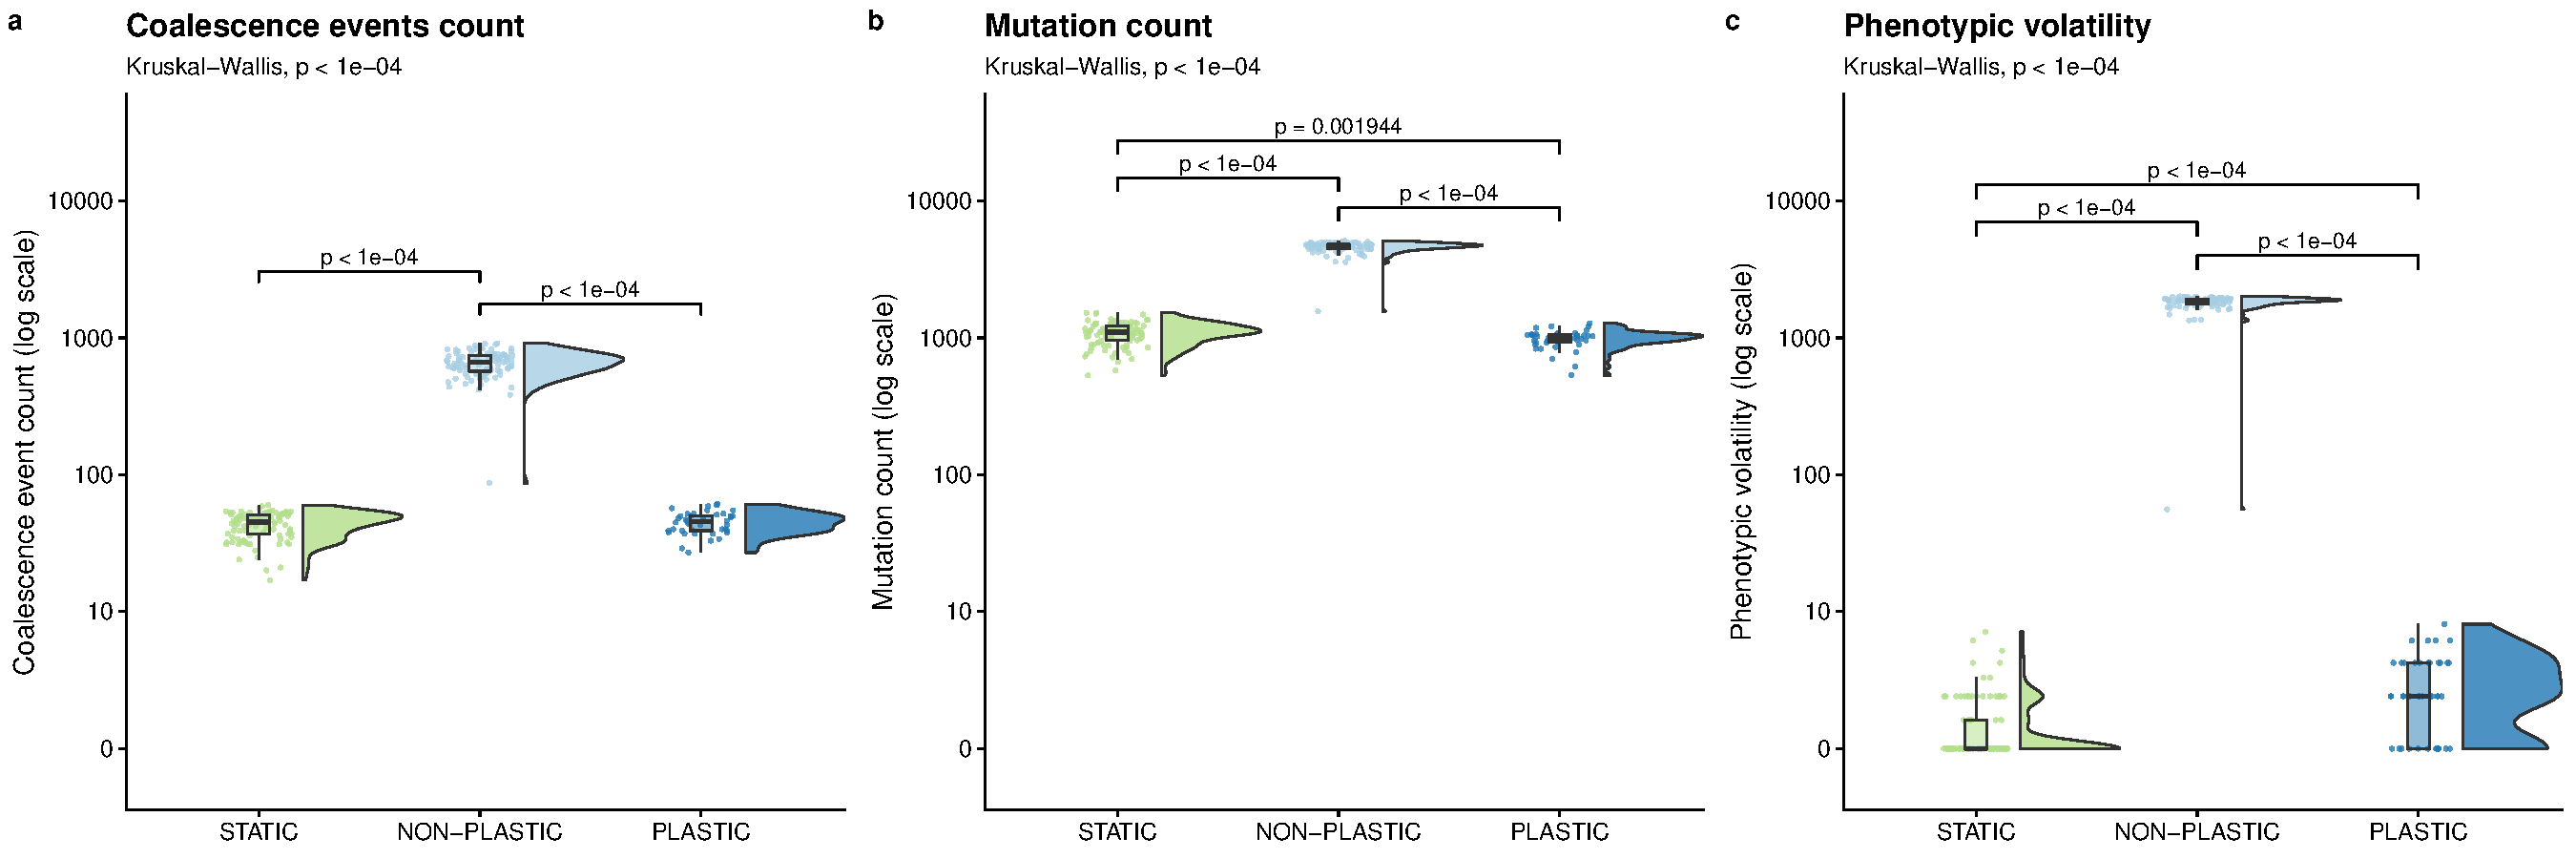
\includegraphics[width=1\textwidth]{media/evolutionary-change-magnitude-panel.pdf}
    \caption{\small
    \textbf{Magnitude of evolutionary change.}
    Raincloud plots \citep{allen_raincloud_2019} of 
    (a) coalescence event count, 
    (b) mutation count, 
    and (c) phenotypic volatility, 
    See Table \ref{tab:metrics-definitions} for descriptions of each metric.
    Each plot is annotated with statistically significant comparisons (Bonferroni-corrected pairwise Wilcoxon rank-sum tests).
    Note that adaptive phenotypic plasticity evolved in \evolutionaryChangeRatePlasticReps\ of \evolutionaryChangeRateReplicates\ replicates from the PLASTIC treatment during phase one of this experiment; we used this more limited group to found the \evolutionaryChangeRatePlasticReps\ phase-two PLASTIC replicates from which we report these PLASTIC data.
    }
    \label{fig:evolutionary-dynamics-magnitude}
\end{figure}


%%%%%%%%%%%%%%%%%%%%%%%%%%%%%%%%%
% Results to report (2021-02-08 experiment)
% ----- GENERATIONS -----
% - average generations elapsed (of a population)
%   - NON-PLASTIC (median: 41768.65) > PLASTIC (median: 31697.65) > STATIC (median: 30839.75)
%   condition     mean    sd
%   <chr>        <dbl> <dbl>
% 1 NON-PLASTIC 41090. 2702.
% 2 PLASTIC     31016. 2615.
% 3 STATIC      30002. 3011.

% 
% ----- SWEEPS -----
% - coalescence events (total)
%   - NON-PLASTIC (median: 663.5) > ( PLASTIC (median: 45.5) ~~ STATIC (median: 45) )
% - Average number of generations between coalescence events (gens / sweeps)
%   - ( PLASTIC (median: 685.001780758557) ~~ STATIC (median: 693.676265008576) ) > NON-PLASTIC (median: 62.0184902295191) 
% 
% ----- PHENOTYPIC VOLATILITY -----
% - phenotypic volatility (total)
%   - i.e., total number of times phenotypes change along lineages
%   - NON-PLASTIC (median: 1868) > PLASTIC (median: 2) > STATIC (median: 0)
% - phenotypic volatility / lineage length
%   - i.e., how often do genomic changes reflect changes in phenotype? 
%   - NON-PLASTIC (median: 0.437) > PLASTIC (median: 0.0022) > STATIC (median: 0)
% - phenotypic volatility / generations
%   - i.e., per-offspring rate of phenotypic changes
%   - NON-PLASTIC (median: 0.0447) > PLASTIC (median: 6.33e-05) > STATIC (median: 0)
% 
% ----- MUTATION ACCUMULATION -----
% - mutation accumulation (total)
%   - NON-PLASTIC (median: 4657.5) > STATIC (median: 1100) > PLASTIC (median: 998.5)
% - mutation accumulation / lineage length
%   - NON-PLASTIC (median: 1.10048311715591) > STATIC (median: 1.03794597464116) > PLASTIC (median: 1.0328599144651) 
% - mutation accumulation / generation
%   - NON-PLASTIC (median: 0.11) > STATIC (median: 0.0368) > PLASTIC (median: 0.0319) 
% 
% ----- MUTATIONAL EFFECTS -----
% - fraction of mutational steps that alter (aggregate) phenotype
%   - NON-PLASTIC (mean: 0.434007, CI [0.4242,  0.4406]) > PLASTIC (mean: 0.002717008, 0.0020,  0.0035) > STATIC (mean: 0.0006788834, CI [0.0004,  0.0009])
% - fraction of phenotype-altering mutation steps that alter unexpressed phenotype (PLASTIC condition only)
%   - mean: 0.8247126 CI [0.7443,  0.8994]
% - fraction of mutations that affect unexpressed phenotype that are deleterious (PLASTIC only)
%   - mean: 0.5172414 CI [0.4402,  0.5977]
% - fraction of mutations that affect unexpressed phenotype that are beneficial (PLASTIC only)
%   - mean: 0.4827586 CI [0.4046,  0.5598]
%%%%%%%%%%%%%%%%%%%%%%%%%%%%%%%%%

% -- Magnitude of evolutionary change --
%  - Selective sweeps
%  - Mutation accumulation
%  - Phenotypic volatility
In experimental phase 2A,
we tested whether adaptive phenotypic plasticity constrained or promoted subsequent evolutionary change in a fluctuating environment. 
First, we compared the total amount of evolutionary change in populations evolved under the PLASTIC, NON-PLASTIC, and STATIC treatments as measured by coalescence event count, mutation count, and phenotypic volatility (Figure \ref{fig:evolutionary-dynamics-magnitude}).
According to each of these metrics, NON-PLASTIC populations experienced a larger magnitude of evolutionary change than either PLASTIC or STATIC populations.
We observed significantly higher coalescence event counts in NON-PLASTIC populations than in PLASTIC or STATIC populations (Figure \ref{fig:evolutionary-dynamics-magnitude}\hyperref[fig:evolutionary-dynamics-magnitude]{a}).
NON-PLASTIC lineages had significantly higher mutation counts (Figure \ref{fig:evolutionary-dynamics-magnitude}b) and phenotypic volatility than PLASTIC or STATIC lineages (Figure \ref{fig:evolutionary-dynamics-magnitude}c).

% -- Elapsed generations --
Changing environments have been shown to increase generational turnover in Avida populations \citep{canino-koning_evolution_2016}, which could explain why we observe a larger magnitude of evolutionary change at the end of 200,000 updates of evolution in NON-PLASTIC populations. 
Indeed, we found that significantly more generations of evolution elapsed in NON-PLASTIC populations (mean of $41090\pm2702$ std. dev.) than in PLASTIC (mean of $31016\pm2615$ std. dev.) or STATIC (mean of $30002\pm3011$ std. dev.) populations during phase 2A (corrected Wilcoxon rank-sum tests, p $<10^{-4}$).

% -- Rate of evolutionary change => intuition --
To evaluate whether increased generational turnover explains the greater magnitude of evolutionary change in NON-PLASTIC populations, we examined the average number of generations between coalescence events and the realized mutational robustness of lineages (Table \ref{tab:metrics-definitions}).
A coalescence event indicates a selective sweep, which is a hallmark of adaptive evolutionary change.
Realized mutational robustness measures the frequency that mutations cause phenotypic changes along a lineage.
We expect that static conditions should favor fit lineages with high realized mutational robustness that no longer undergo rapid adaptive change and hence do not trigger frequent coalescence events.
Under fluctuating conditions, however, lineages must be composed of plastic organisms if they are to maintain both high fitness and realized mutational robustness.
Without plasticity, we expect fluctuating conditions to produce lineages with low realized mutational robustness and frequent coalescence events as populations must continually acquire and fix mutations to readapt to the environment.  


\begin{figure}[h!]
    \centering
    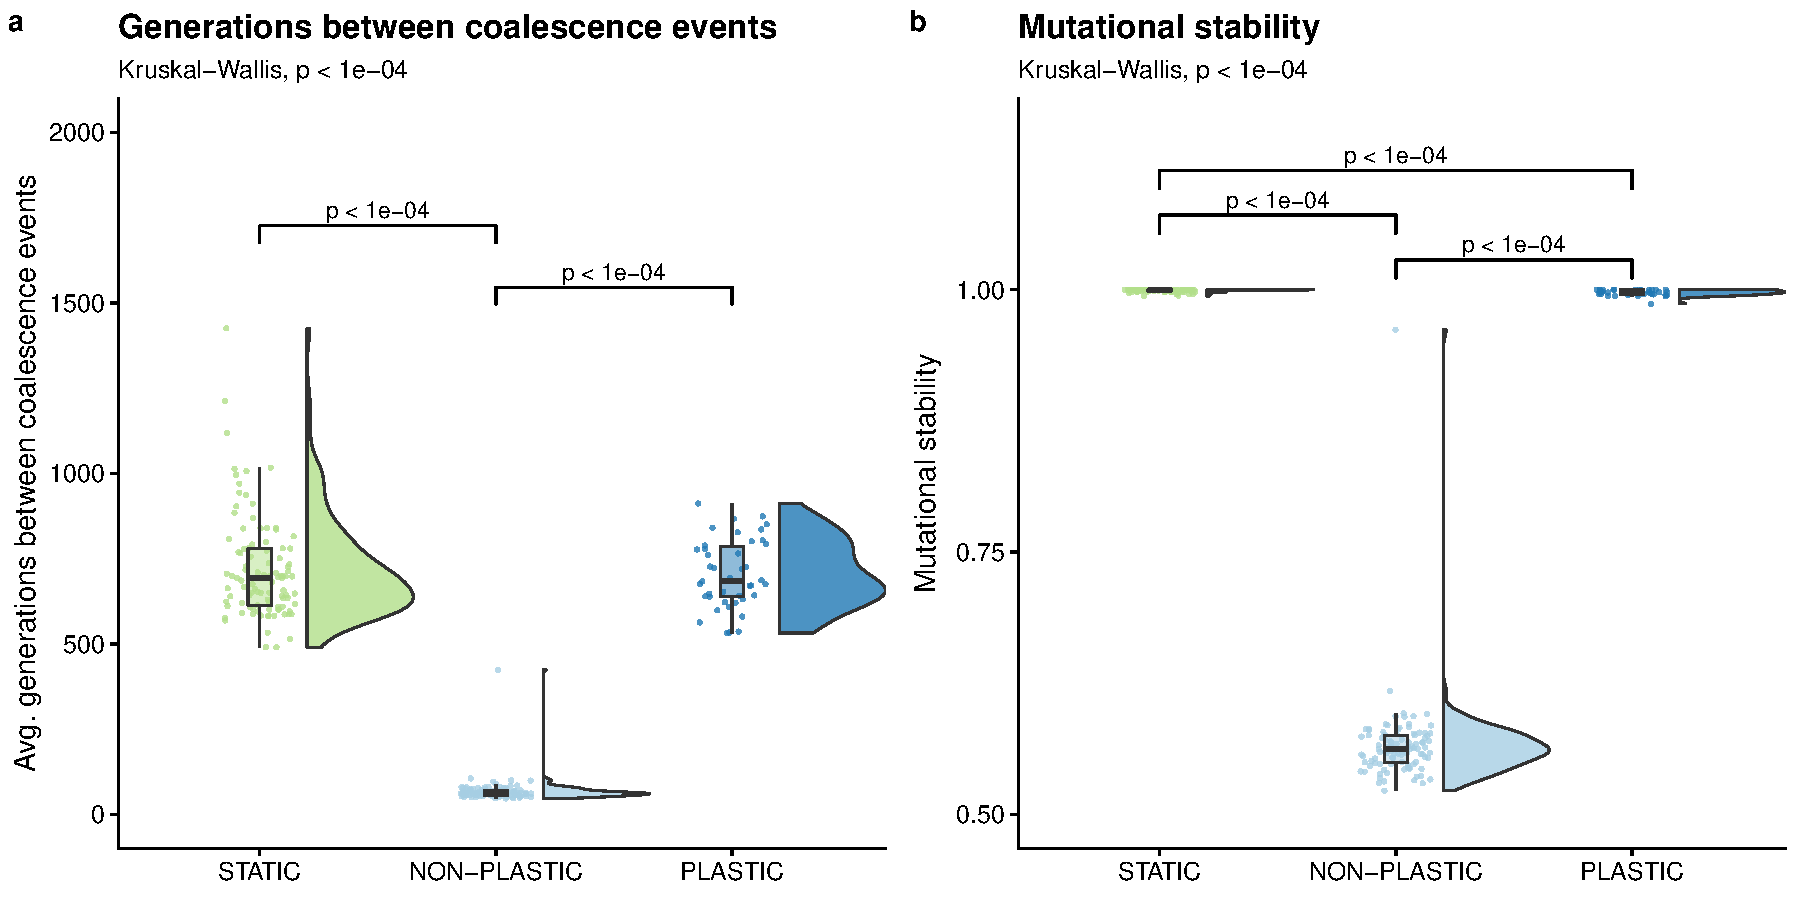
\includegraphics[width=0.66\textwidth]{media/evolutionary-change-pace-panel.pdf}
    \caption{\small
    \textbf{Pace of evolutionary change.}
    Raincloud plots of 
    (a) average number of generations between coalescence events,
    and (b) mutational stability (Table \ref{tab:metrics-definitions}).
    Each plot is annotated with statistically significant comparisons (Bonferroni-corrected pairwise Wilcoxon rank-sum tests).
    }
    \label{fig:evolutionary-dynamics-rate}
\end{figure}

% -- Rate of evolutionary change => findings --
On average, significantly fewer generations elapsed between coalescence events in NON-PLASTIC populations than in either PLASTIC or STATIC populations (Figure \ref{fig:evolutionary-dynamics-rate}a).
We also found that both STATIC and PLASTIC lineages exhibited higher realized mutational robustness relative to that of NON-PLASTIC lineages (Figure \ref{fig:evolutionary-dynamics-rate}b); that is, mutations observed along NON-PLASTIC lineages more often caused phenotypic changes in offspring. 
Overall, our results indicate that NON-PLASTIC populations underwent more rapid (and thus a greater amount of) evolutionary change than either PLASTIC or STATIC populations. 

% -- Mutational stability in static and plastic lineages --
While both STATIC and PLASTIC lineages exhibited high realized mutational robustness, we found that STATIC lineages exhibited higher realized robustness than PLASTIC lineages (Figure \ref{fig:evolutionary-dynamics-rate}b). 
Overall, there were rare instances of mutations that caused a change in phenotypic profile across all PLASTIC lineages.
Of these mutations, we found that over 80\% (83 out of 102) of changes to phenotypic profiles were cryptic. 
That is, the mutations affected traits that would not have been expressed in the environment that the organism was born into but would have been expressed had the environment changed.

%\begin{figure}[h!]
    \centering
    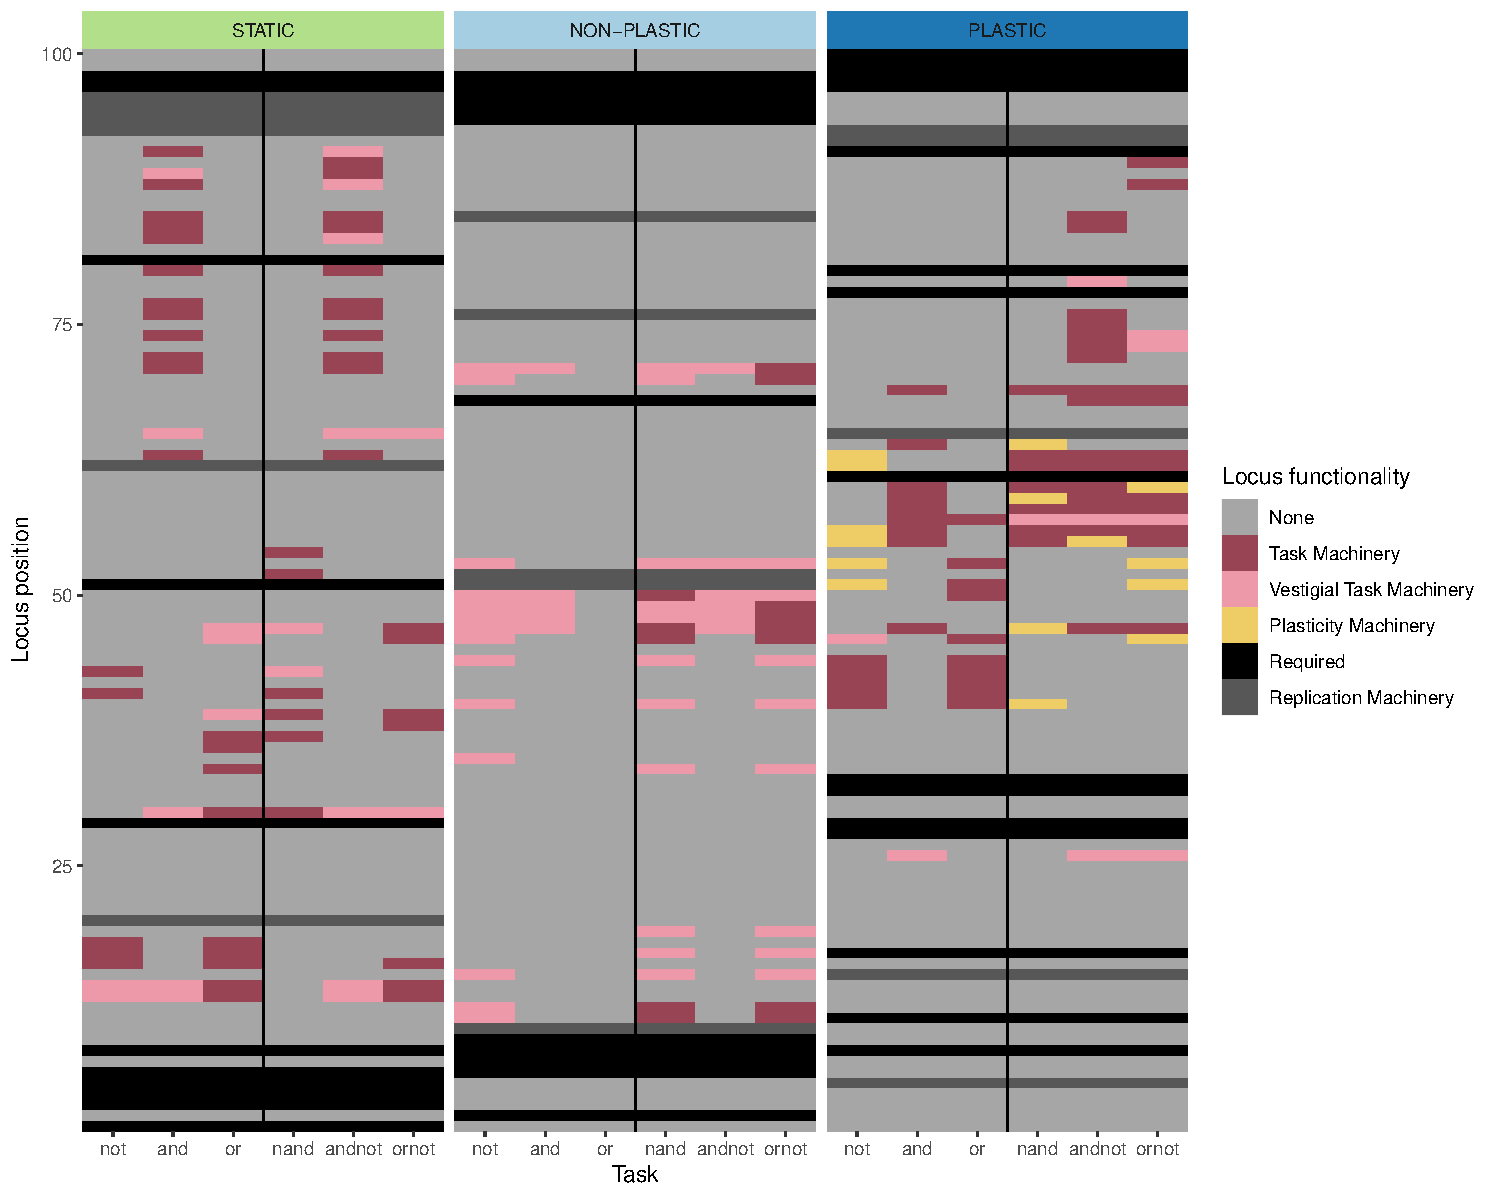
\includegraphics[width=1\textwidth]{media/architecture/locus_slice_combined_color_facets.pdf}
    \caption{\small
    % TODO: Change "Previous Task Machinery" -> "Vestigial Task Machinery"
    \textbf{Locus functionality.}
    Each box shows a representative genome from each condition at the end of Phase 2A. 
    The y-axis indicates each site in each genome, and colors indicate the function of each locus with respect to a particular task (given by the x-axis). 
    % Each of the six base tasks are shown on the x axis. 
    The vertical black line splits tasks rewarded in ENV-A (left of the line) from those rewarded in ENV-B.
    Loci colored as ``Task Machinery'' are actively involved in the performance of that task, while ``Vestigial Task Machinery'' represents loci that have not mutated, but no longer code for the task (\textit{i.e.}, a change elsewhere in the genome has disabled or modified the task). 
    ``Plasticity Machinery'' refers to loci that regulate the given task. 
    Knocking out a ``Replication Machinery'' locus negatively affects replication time, while knocking out a ``Required'' locus results in a non-viable organism. 
    }
    \label{fig:architecture_locus_functionality}
\end{figure}

% @AML: Original caption:
    % Each box shows a representative sample from each condition at the end of Phase 2A. 
    % The 100-loci genome of each sample is shown on the y axis, with colors indicating function of each locus has for each of the six base tasks. 
    % Each of the six base tasks are shown on the x axis. 
    % The vertical black line splits tasks rewarded in ENV-A (right of the line) from those rewarded in ENV-B.
    % Loci colored as Task Machinery are actively involved in the performance of that task, while Vestigial Task Machinery represents loci that have not mutated, but no longer code for the task (i.e., a change elsewhere in the genome has disabled or modified the task). 
    % Plasticity Machinery refers to loci that prevent the task from occurring in both the A and B environments. 
    % Knocking out a Replication Machinery locus will have a substantial negative effect on replication time, while knocking out a Required locus results in a non-viable organism. 

%\begin{figure}[ht!]
    \centering
    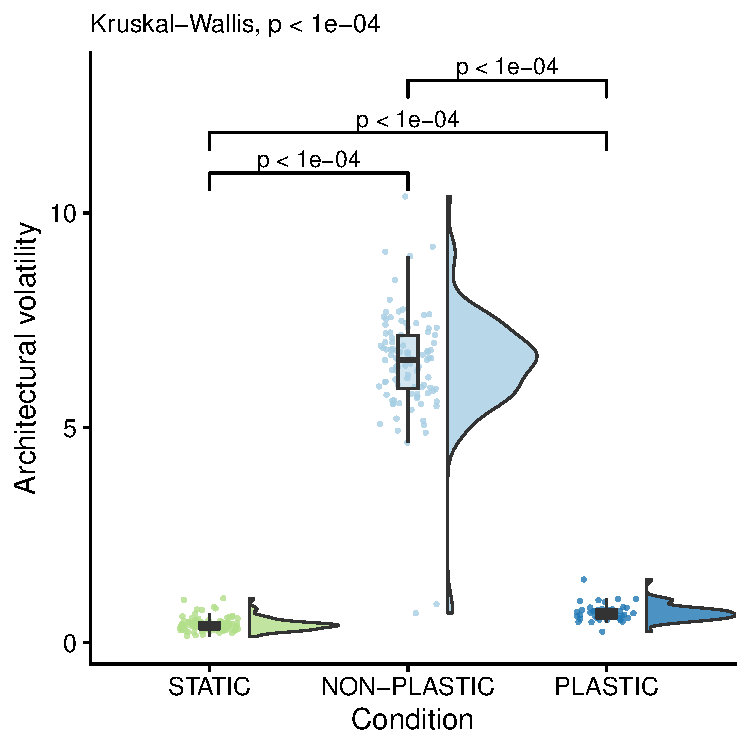
\includegraphics[width=0.33\textwidth]{media/architecture/architectural_volatility.pdf}
    \caption{\small
        \textbf{Architectural volatility.}
        Raincloud plot of architecture volatility (Table \ref{tab:metrics-definitions}).
        The plot is annotated with statistically significant comparisons (Bonferroni-corrected pairwise Wilcoxon rank-sum tests). 
    }
    \label{fig:architecture_volatility}
\end{figure}
%\begin{figure}[h!]
    \centering
    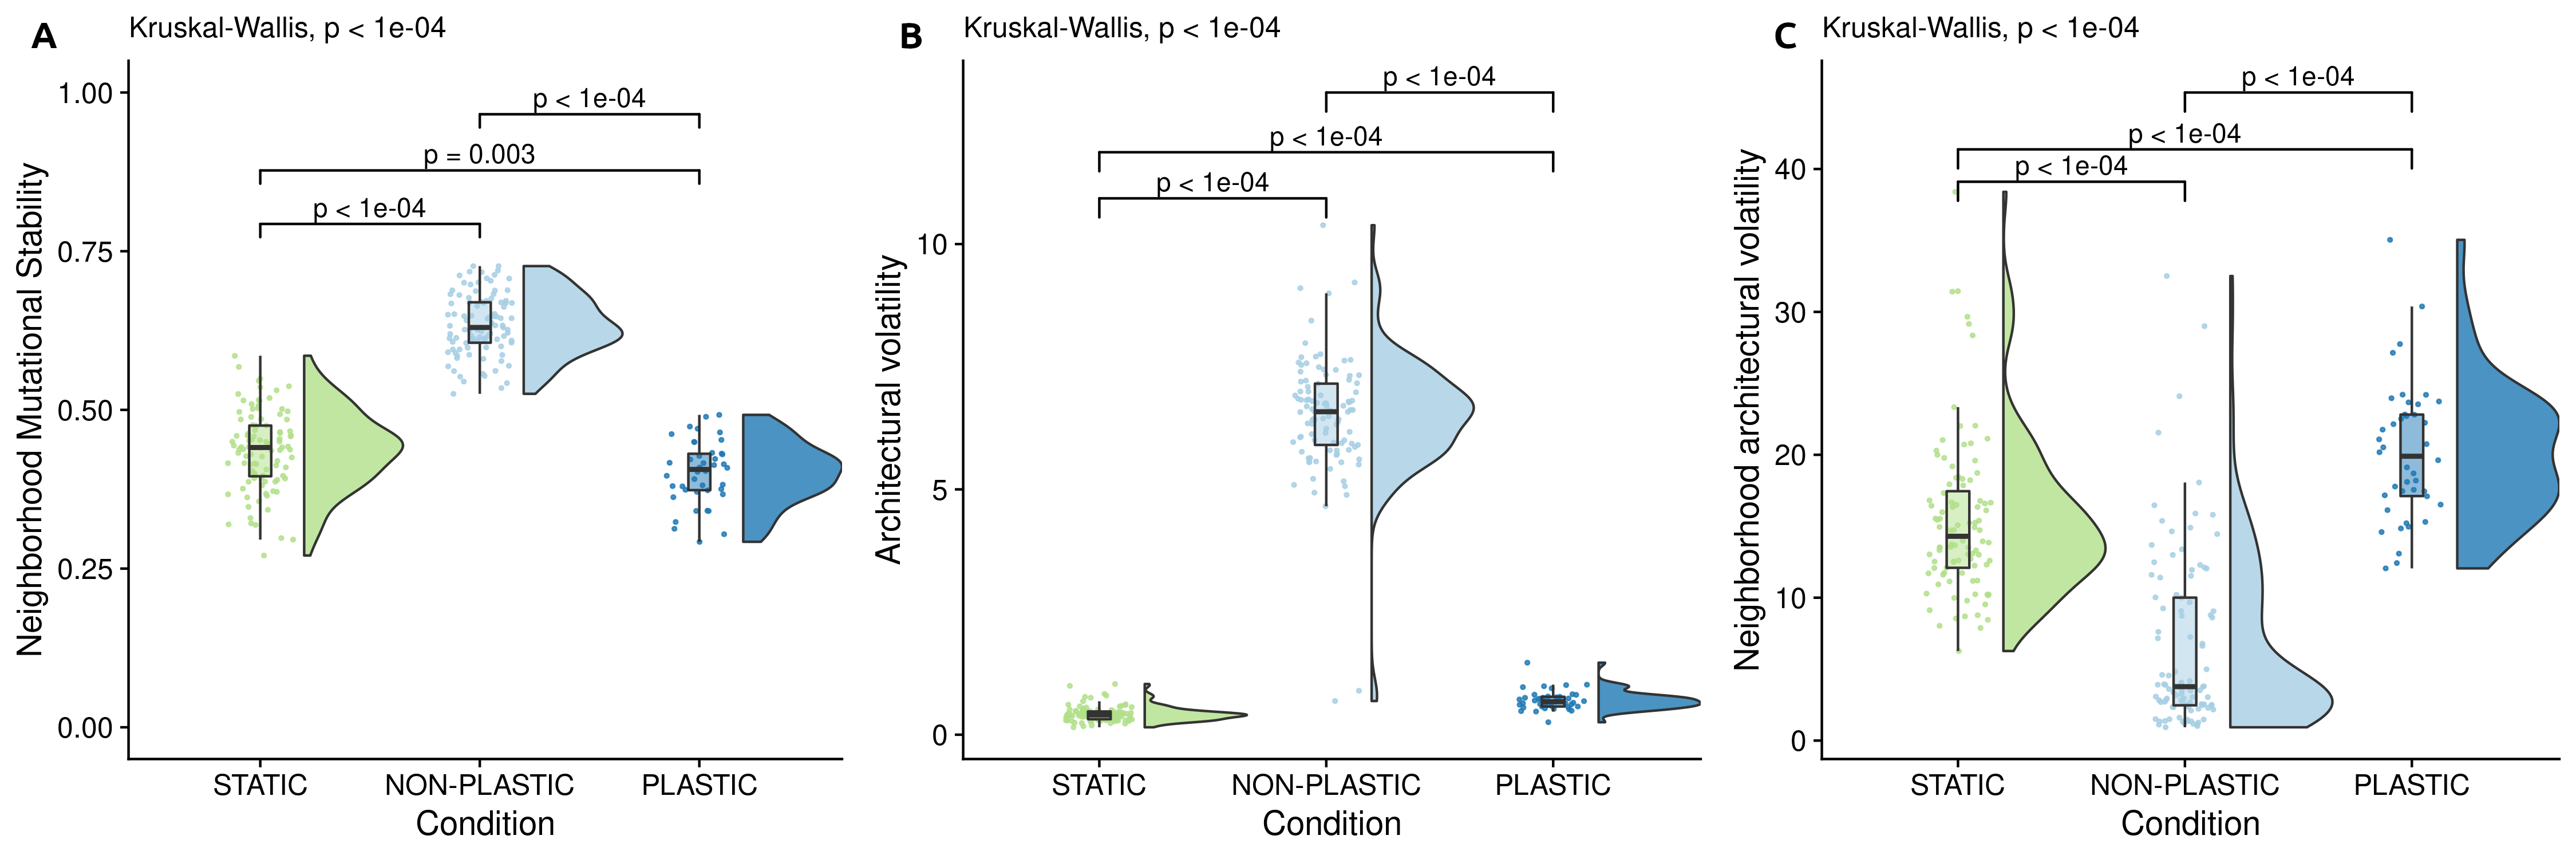
\includegraphics[width=1\textwidth]{media/architecture/quick_architecture_panel.png}
    \caption{\small
    \textbf{todo.}
    Raincloud plots \citep{allen_raincloud_2019} of 
    (a) neighborhood mutational stability, 
    (b) lineage architectural volatility, 
    and (c) neighborhood architectural volatility. 
    See Table \ref{tab:metrics-definitions} for descriptions of each metric.
    Each plot is annotated with statistically significant comparisons (Bonferroni-corrected pairwise Wilcoxon rank-sum tests).
    }
    \label{fig:architecture-panel}
\end{figure}
\begin{figure}[ht!]
    \centering
    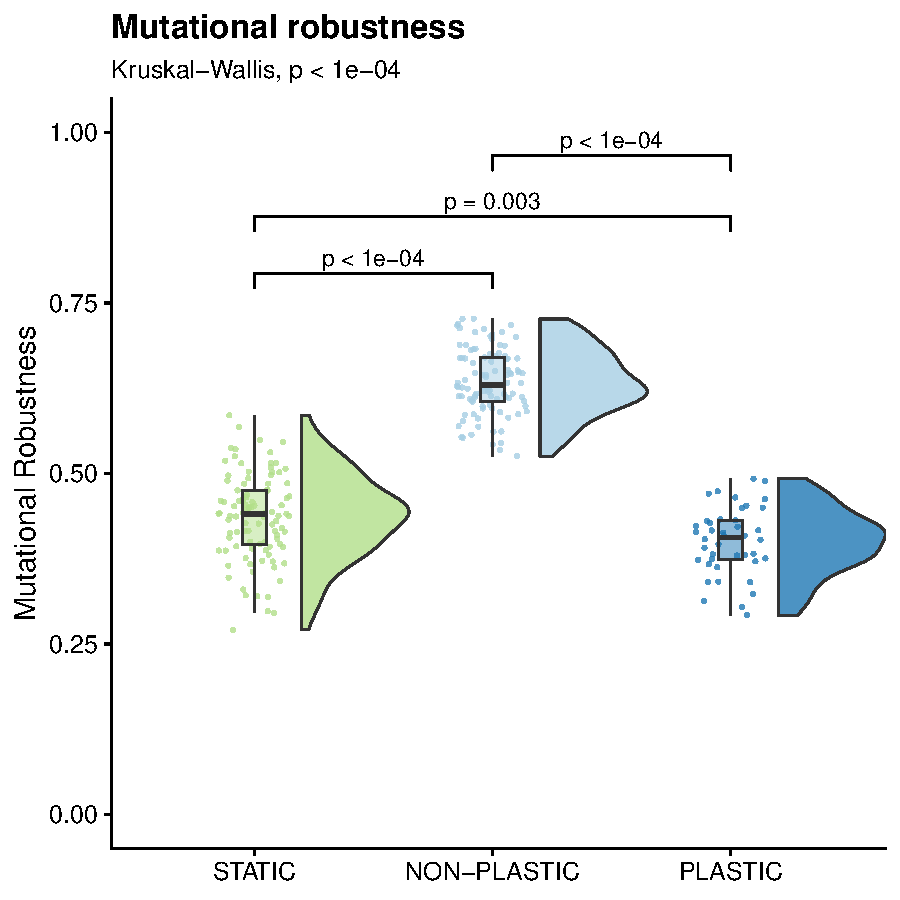
\includegraphics[width=0.33\textwidth]{media/mutational_robustness.pdf}
    \caption{\small
        \textbf{Mutational robustness.}
        Raincloud plot of mutational robustness of each representative genotype (Table \ref{tab:metrics-definitions}).
        The plot is annotated with statistically significant comparisons (Bonferroni-corrected pairwise Wilcoxon rank-sum tests). 
    }
    \label{fig:mutational-robustness}
\end{figure}

% -- mutational landscaping --
% Thus far, our analyses have focused on dominant lineage.
% What about mutations off the line of descent? 
% Mutational stability result is NOT due to random mutations being more likely to induce phenotypic change. 
% KEY: Motivation for looking at mutational neighborhoods needs to made very clear here
%   - Why not look at mutational neighborhoods for the other experiments?
Given that NON-PLASTIC lineages exhibited the lowest realized mutational robustness of our three experimental treatments, we sought to determine if this effect was driven by differences in evolved genetic architectures.
Specifically, did the NON-PLASTIC genetic architectures evolve such that mutations were more likely to result in phenotypic change?
Such a  mutational bias would trade off descendant fitness in the same environment in exchange for a chance of increasing descendant fitness in alternate environments.
This strategy would be an example of diversifying bet-hedging (\textit{i.e.}, reducing expected mean fitness to lower variance in fitness) \citep{childs2010evolutionary}.
Alternatively, the lower realized mutational robustness in NON-PLASTIC lineages could be due to survivorship bias, as we measured realized mutational robustness as the fraction of mutations observed along \textit{successful} lineages that caused a phenotypic change. 
%(\textit{i.e.}, the lineages of extant organisms) 


We analyzed the mutational robustness of representative genotypes by calculating the fraction of single-instruction mutations that change the phenotypic profile.
We found that mutations to representative genotypes on NON-PLASTIC lineages are \textit{less} likely to result in a phenotypic change than mutations to comparable genotypes on either STATIC or PLASTIC lineages (Figure \ref{fig:mutational-robustness}).
These data provide evidence against NON-PLASTIC lineages engaging in a mutation-driven bet-hedging strategy, and instead, are consistent with the hypothesis that lower realized mutational robustness in the NON-PLASTIC treatment was due to survivorship bias.
% @AML: Maybe one more sentence elaborating on implication of survivorship bias?

% -- in general, PLASTIC and STATIC more similar than NON-PLASTIC --
In general, adaptive plasticity stabilized PLASTIC-treatment populations against environmental fluctuations, and their evolutionary dynamics more closely resembled those of populations evolving in a static environment.
We observed no significant difference in the number and frequency of coalescence events in PLASTIC and STATIC populations.
We did, however, observe small, but statistically significant, differences in each of the following metrics: elapsed generations, mutation counts, mutational robustness, and realized mutational robustness between PLASTIC and STATIC populations. 

\vspace{0.5cm}
\subsection{Adaptively plastic populations retain more novel tasks than non-plastic populations in fluctuating environments}

%%%%%%%%%%%%%%%%%%%%%%%%%%%%%%%%%
% Results to report (2021-01-31)
% - Number of plastic replicates
% - Final dominant genotype # novel traits
%   - non-plastic < (plastic == static)
% - Final population (1% threshold): 
%   - non-plastic < plastic < static
% - Final population (1% threshold) discovered:
%   - non-plastic > (plastic ~~ static)
% - Lineage tasks discovered
%   - non-plastic > static ~>(nosig) plastic
% - Lineage tasks discovered / step
%   - (static ~~ plastic) > non-plastic 
% - Lineage tasks lost
%   - non-plastic > static > plastic
% - Lineage tasks lost / step
%   - non-plastic > static > plastic

% - tasks discovered per generation(?)
%   - NON-PLASTIC [0.00014358046266055] ~~ STATIC [0.00015363220504867] > PLASTIC [0.000117695011124939]
% - tasks lost per generation(?)
%   - NON-PLASTIC [0.0022026054610079] > STATIC [0.000161396283669756] > PLASTIC [6.25141973661864e-05]
%%%%%%%%%%%%%%%%%%%%%%%%%%%%%%%%%

\begin{figure}[h!]
    \centering
    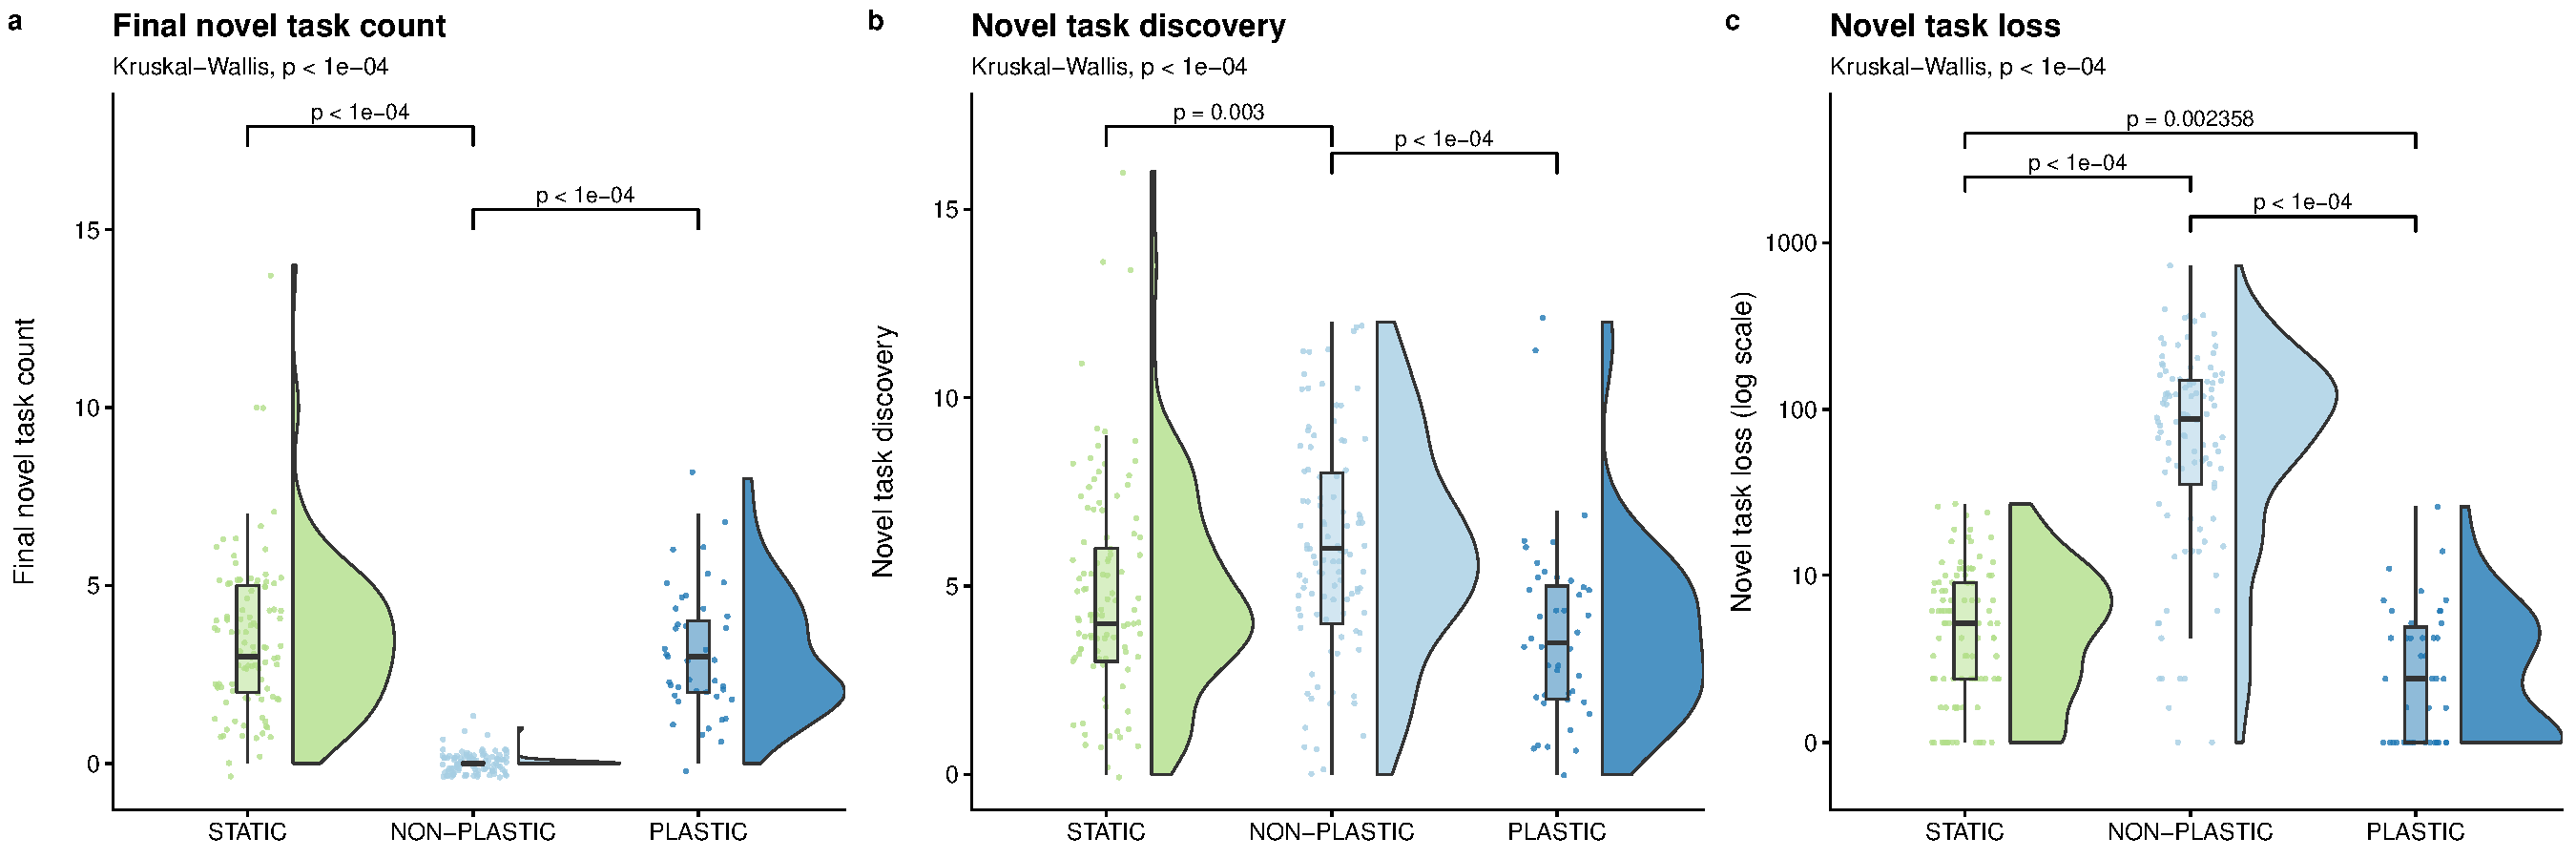
\includegraphics[width=0.9\textwidth]{media/complex-traits-magnitude-panel.pdf}
    \caption{\small
    \textbf{Novel task evolution.}
    Raincloud plots of 
    (a) final novel task count,
    (b) novel task discovery,
    and (c) novel task loss.
    See Table \ref{tab:metrics-definitions} for descriptions of each metric.
    Each plot is annotated with statistically significant comparisons (Bonferroni-corrected pairwise Wilcoxon rank-sum tests).
    Note that adaptive phenotypic plasticity evolved in \novelTraitsPlasticReps\ of \novelTraitsReplicates\ replicates from the PLASTIC treatment during phase one of Experiment II; we used this more limited group to seed the resulting \novelTraitsPlasticReps\ phase-two PLASTIC replicates.
    }
    \label{fig:complex-traits-magnitude}
\end{figure}

% -- What did we test? --
%In experimental phase 2B, we evaluated how evolution of adaptive phenotypic plasticity influences the ability of populations to evolve and retain novel adaptive traits. Commented out by Nkrumah... 
We have so far shown that adaptive plasticity constrains the rate of evolutionary change in fluctuating environments.
However, it is unclear how this dynamic influences the evolution of novel tasks.
Based on their relative rates of evolutionary change, we might expect NON-PLASTIC-treatment populations to evolve more novel tasks than PLASTIC-treatment populations.
But, how much of the evolutionary change in NON-PLASTIC populations is useful for exploring novel regions of the fitness landscape versus continually rediscovering the same regions?

% - Magnitude of exploration/exploitation -
To answer this question, we quantified the number of novel tasks performed by a representative organism in the final population of each replicate.
We found that both PLASTIC and STATIC populations had significantly higher final task counts than NON-PLASTIC populations at the end of the experiment (Figure~\ref{fig:complex-traits-magnitude}a). 
The final novel task count in PLASTIC and STATIC lineages could be higher than that of the NON-PLASTIC lineages for several non-mutually exclusive reasons. 
One possibility is that PLASTIC and STATIC lineages could be exploring a larger area of the fitness landscape when compared to NON-PLASTIC lineages. 
Another possibility is that the propensity of the NON-PLASTIC lineages to maintain novel traits could be significantly lower than PLASTIC or STATIC lineages. 
When we looked at the total sum of novel tasks discovered by each of the PLASTIC, STATIC, and NON-PLASTIC lineages, we found that NON-PLASTIC lineages generally explored a larger area of the fitness landscape (Figure~\ref{fig:complex-traits-magnitude}b).
Although the NON-PLASTIC lineages discovered more novel tasks, those lineages also exhibited significantly higher novel task loss when compared to PLASTIC and STATIC lineages (Figure~\ref{fig:complex-traits-magnitude}c). 

\begin{figure}[h!]
    \centering
    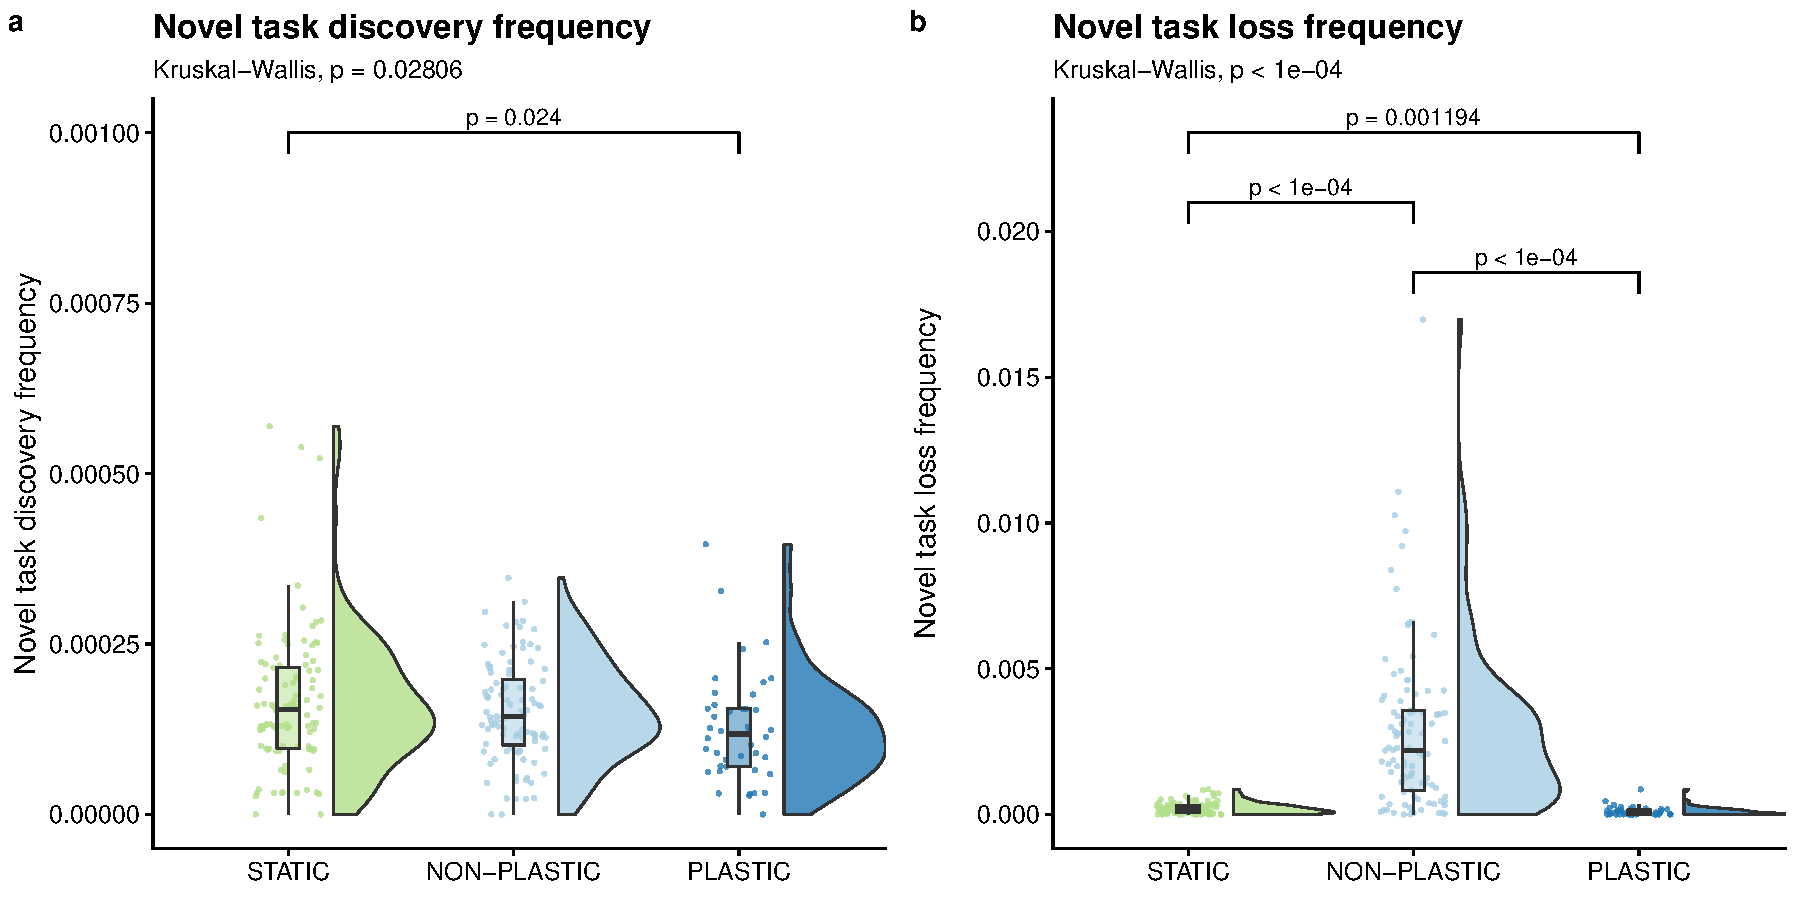
\includegraphics[width=0.66\textwidth]{media/complex-traits-pace-panel.pdf}
    \caption{\small
    \textbf{Rate of novel task evolution.}
    Raincloud plots of 
    (a) novel task discovery frequency
    and (b) novel task loss frequency.
    Each plot is annotated with statistically significant comparisons (Bonferroni-corrected pairwise Wilcoxon rank-sum tests).
    }
    \label{fig:complex-traits-rate}
\end{figure}

% - Rates of exploration/exploitation -
A larger number of generations elapsed in NON-PLASTIC populations than in PLASTIC or STATIC populations during our experiment \citep{supplemental_material}.
Are NON-PLASTIC lineages discovering and losing novel tasks more frequently than PLASTIC or STATIC lineages, or are our observations a result of differences in generational turnover?
To answer this question, we converted the metrics of novel task discovery and novel task loss to rates by dividing each metric by the number of elapsed generations along the associated representative lineages.
We found no significant difference in the frequency of novel task discovery between NON-PLASTIC and STATIC lineages, and we found that PLASTIC lineages had a lower frequency of novel task discovery than STATIC lineages (Figure~\ref{fig:complex-traits-rate}a).
Therefore, we cannot reject the possibility that the larger magnitude of task discovery in NON-PLASTIC lineages was driven by a larger number of elapsed generations.
NON-PLASTIC lineages had a higher frequency of task loss than either PLASTIC or STATIC lineages, and PLASTIC lineages tended to have a lower frequency of novel task loss than STATIC lineages (Figure~\ref{fig:complex-traits-rate}b). 


% - Characterizing trait loss -
Next, we examined the frequency at which novel task loss along lineages co-occurred with the loss or gain of any of the six base tasks.
Across all NON-PLASTIC representative lineages, over 97\% (10998 out of 11229) of instances of novel task loss co-occurred with a simultaneous change in base task profile.
In contrast, across all PLASTIC and STATIC dominant lineages, we observed that approximately 20\% (29 out of 142) and 2\% (13 out of 631), respectively, of instances of novel task loss co-occurred with a simultaneous change in base task profile.
As such, the losses of novel tasks in NON-PLASTIC lineages appear to be primarily due to hitchhiking.

\subsection{Lineages without plasticity that evolve in fluctuating environments express more deleterious tasks}

%%%%%%
% 2021-02-05 - Results
% - Number of offspring on lineage where hitchhiker instruction execution increases (i.e., instances of hitchhiking)
%   - PLASTIC ~~ STATIC < NON-PLASTIC
% - Hitchhiker instruction increases / offspring on lineage
%   - PLASTIC ~~ STATIC < NON-PLASTIC
% - What fraction of mutations that increase hitchhiker instruction execution co-occur with base trait changes?
%   - NON-PLASTIC > PLASTIC ~~ STATIC
% - What about unexpressed vs expressed trait changes in plastic populations? (plastic only)
%   - Not much hitchhiking. Did not find evidence that hitchiking occurring as cryptic variation in unexpressed phenotype.
%%%%%%

Phenotypic plasticity allows for genetic variation to accumulate in genomic regions that are unexpressed, which could lead to the fixation of deleterious instructions in PLASTIC populations.
However, in NON-PLASTIC lineages, we observe a higher rate of novel task loss, indicating that they may be more susceptible to deleterious mutations (Figure \ref{fig:complex-traits-rate}b).

Therefore, in experiment phase 2C, we tested whether adaptive phenotypic plasticity can increase the incidence of deleterious task performance. 
Specifically, we added an instruction that triggered a ``poisonous'' task and measured the number of times it was executed.
Each execution of the  \code{poison} instruction reduces an organism's fitness by 10\%. 
At the beginning of phase 2C, the \code{poison} instruction is not present in the population, as it was not part of the instruction set during phase one of evolution.
Accordingly, if a \code{poison} instruction fixes in a population, it must be the result of evolutionary dynamics during phase 2C, including cryptic variation or hitchhiking. 

\begin{figure}[ht!]
    \centering
    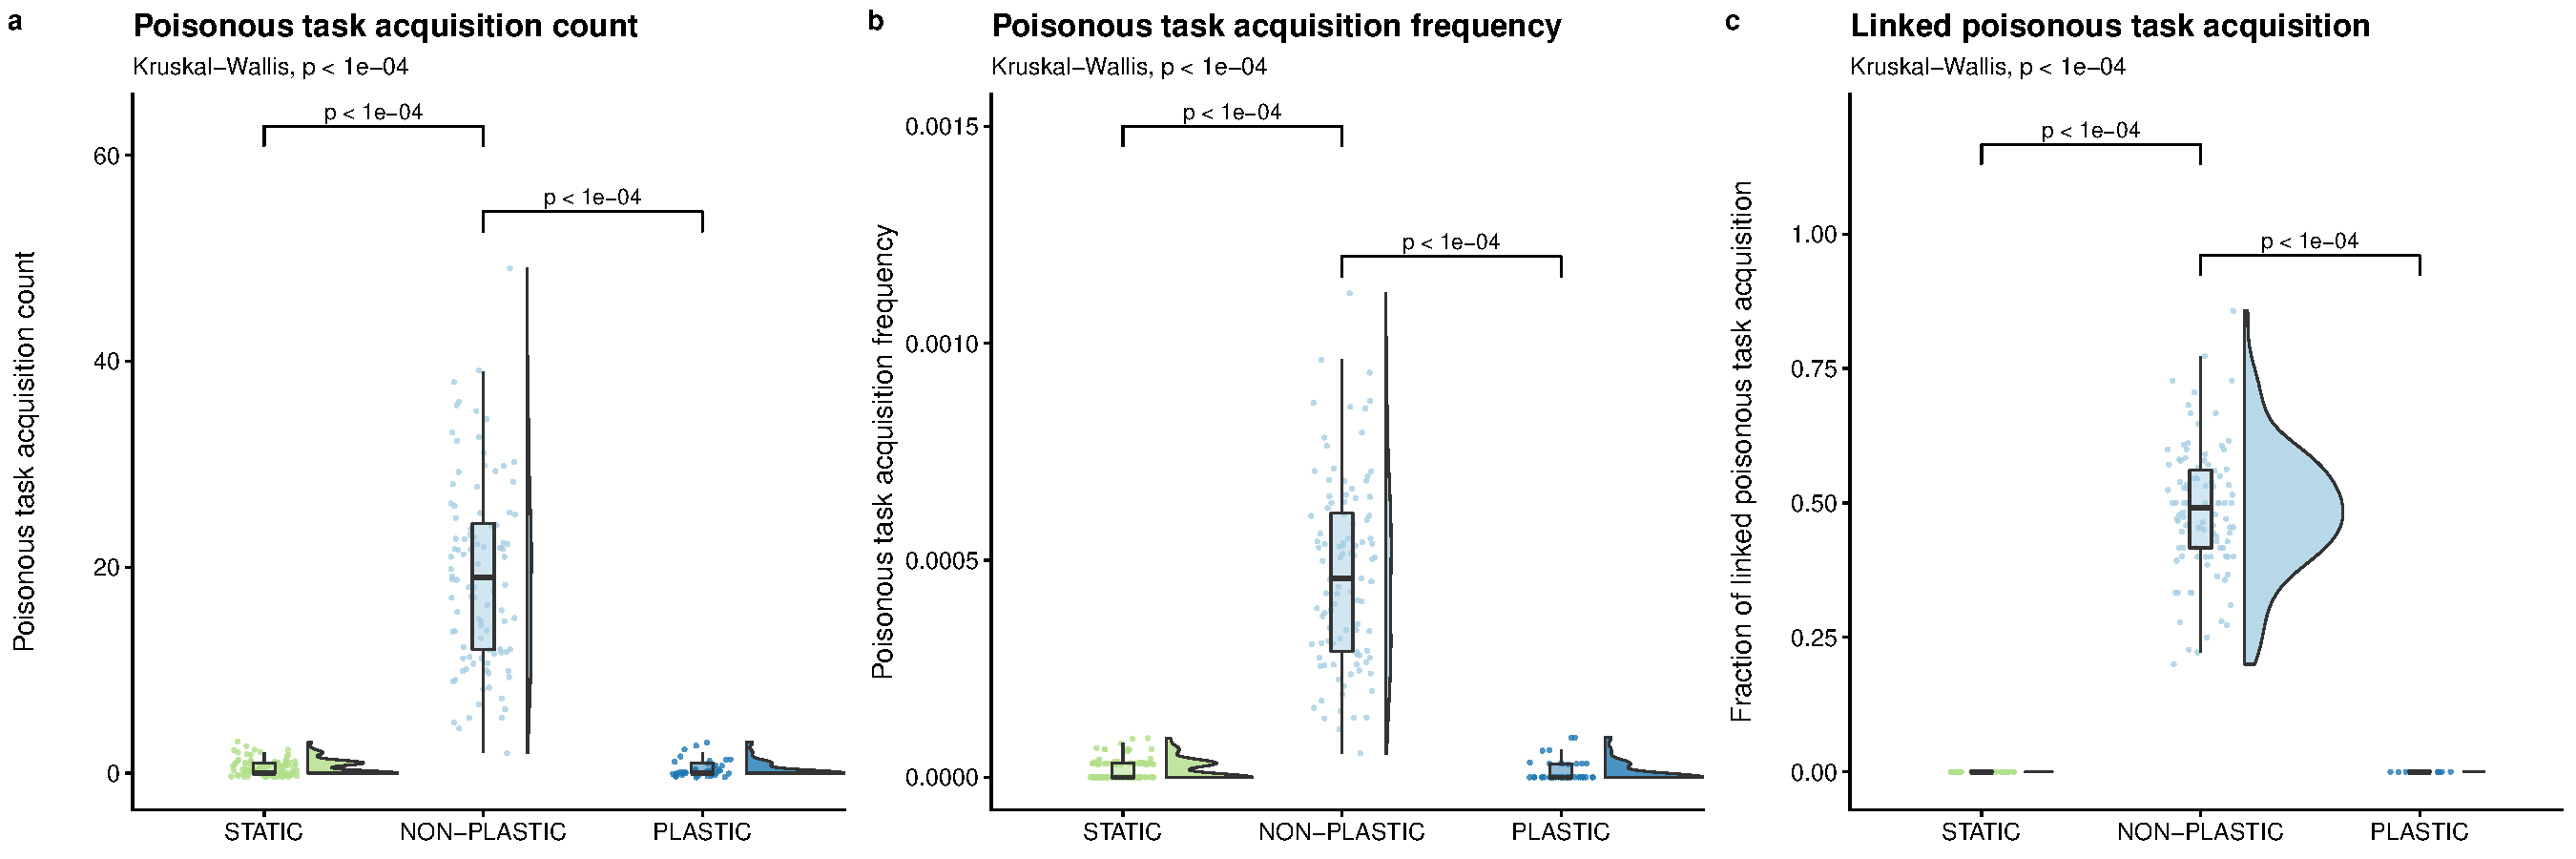
\includegraphics[width=1.0\textwidth]{media/poison-accumulation-panel.pdf}
    \caption{\small
    \textbf{Deleterious instruction accumulation.}
    Raincloud plots of 
    (a) poisonous task acquisition,
    (b) poisonous task acquisition frequency,
    and (c) the proportion of mutations that increase poisonous task performance along a lineage that co-occur with another change in phenotypic profile.
    Each plot is annotated with statistically significant comparisons (Bonferroni-corrected pairwise Wilcoxon rank-sum tests).
    Note that adaptive phenotypic plasticity evolved in \deleteriousHitchhikingPlasticReps\ of \deleteriousHitchhikingReplicates\ replicates from the PLASTIC treatment during phase one of Experiment III; we used this more limited group to seed the \deleteriousHitchhikingPlasticReps\ phase-two PLASTIC replicates.
    }
    \label{fig:deleterious-hitchhiking}
\end{figure}

% -- Instruction execution by final dominant & along lineage --
At the end of our experiment, no representative organisms from the PLASTIC or STATIC treatments performed the poisonous task under any environmental condition; however, representative organisms in 14\% of replicates of the NON-PLASTIC treatment performed the poisonous task at least once. 
NON-PLASTIC lineages contained significantly more mutations that conferred the poisonous task as compared to PLASTIC or STATIC lineages (Figure \ref{fig:deleterious-hitchhiking}a), and these mutations occurred at a significantly higher frequency in NON-PLASTIC lineages (Figure \ref{fig:deleterious-hitchhiking}b).
% Additionally, we did not observe 
% This result does not change when we normalize [what?] by the number of generations represented in the given lineage (Figure \ref{fig:deleterious-hitchhiking}b).

% -- When/where does hitchhiking take place? --
Next, we measured how often mutations that increased poisonous task performance co-occurred with changes to the base task profile within representative lineages.
A poisonous instruction can fix in a lineage by having a beneficial effect that outweighs its inherent cost (\textit{e.g.}, knocking out a punished task) or through linkage with a secondary beneficial mutation at another site within the genome.
Across all NON-PLASTIC representative lineages, we found that approximately 49\% (956 out of 1916) of mutations that increased poisonous task expression co-occurred with a change in the base task profile (Figure \ref{fig:deleterious-hitchhiking}c).
In all representative lineages from the PLASTIC treatment, only 18 mutations increased poisonous task expression, and none co-occurred with a change in base task profile (Figure \ref{fig:deleterious-hitchhiking}c).
Likewise, only 58 mutations increased poisonous task performance in all representative lineages from the STATIC treatment, and none co-occurred with a change in base task profile (Figure \ref{fig:deleterious-hitchhiking}c).
We did not find compelling evidence that the few mutations that increased poisonous task expression occurred as cryptic variation in PLASTIC lineages.

We repeated this experiment with 3\% and 30\% metabolic rate penalties associated with the poisonous task, which produced results that were consistent with those reported here \citep{supplemental_material}.

% GUIDELINES:
% This section may be divided by subheadings. Discussions should cover the key findings of the study: discuss any prior research related to the subject to place the novelty of the discovery in the appropriate context, discuss the potential shortcomings and limitations on their interpretations, discuss their integration into the current understanding of the problem and how this advances the current views, speculate on the future direction of the research, and freely postulate theories that could be tested in the future.

%%%%%%%%%%%
% Would be nice to have empirical studies/relevant examples about:
% --- Evolutionary change ----
% - how repeated bouts of directional selection affect evolutionary change (mutation accumulation/phenotypic volatility/sweeps)
% - Adaptive plasticity can stabilize populations against fluctuations
% - Relaxed selection in plastic genes (or difficulty in maintaining costly plasticity)
% --- Novel traits ----
% - changing environments + fitness landscape exploration
% - plasticity stabilizes populations => allows further adaptation
% --- Deleterious genes ----
%%%%%%%%%%%

%%%%%%%%%
% Text to work in:

% -- coalescence times --
% In asexual populations without ecological interactions fostering coexistence, phylogenies should coalesce periodically; that is, the most recent common ancestor shared by the extant population should change.
% The rate that these coalescence events occur can indicate the strength of selection.
% For example, populations under strong selective pressures should experience more rapid coalescence events than populations under weaker selection \citep{dolson_interpreting_2020}.

% The rate that coalescence events occur can indicate the strength of selection \citep{dolson_interpreting_2020}.
% For example, we would expect populations evolving under strong directional selective pressures to experience more rapid coalescence events than populations evolving under weak selective pressures.

%%%%%%%%%


\section{Discussion}

In this work, we used evolving populations of digital organisms to determine how adaptive phenotypic plasticity alters subsequent evolutionary dynamics and influences evolutionary outcomes in fluctuating environments.
First, we examined the evolutionary histories of plastic and non-plastic populations to test whether the evolution of adaptive plasticity promotes or constrains subsequent evolutionary change.
Next, we evaluated how adaptive plasticity influences fitness landscape exploration and exploitation by testing whether plastic populations are better able to evolve and then maintain novel traits.
Finally, we tested if the evolution of adaptive plasticity increases the potential for deleterious instructions to accumulate in evolving genomes.

Overall, our results indicate that adaptive plasticity can improve evolution's ability to maintain and refine novel traits, though with the tradeoff of reducing evolutionary exploration of the fitness landscape.
Additionally, we found no evidence that adaptive plasticity increased the potential for deleterious instructions to accumulate in genomes.
Instead, the genomes of non-plastic organisms that evolved in an identical fluctuating environment accumulated more deleterious instructions than that of the genomes of adaptively plastic organisms. 
These dynamics appear to be driven by the stabilizing effect that adaptive plasticity had on population dynamics rather than plasticity's effect on genetic architecture or regulation.
% Below we discuss the specific implications of the results from each of our three experiments.

\vspace{0.25cm}
\subsection{The rate of evolutionary change}

% -- Adaptively plastic populations underwent less evolutionary change than non-plastic populations --
Adaptively plastic populations experienced fewer selective sweeps and fewer total genetic changes relative to non-plastic populations evolving under the same environmental conditions (Figure \ref{fig:evolutionary-dynamics-magnitude}).
Plastic populations adapted to the fluctuating environmental regime by evolving to sense environmental changes and regulate their metabolism (task performance) in response to such changes, which also stabilized these populations against fluctuations.
Indeed, across all three of our experiments, the evolutionary dynamics of plastic populations were more similar to that of populations evolving in a static environment than to that of non-plastic populations evolving in an identical fluctuating environment.

% -- Non-plastic populations repeatedly re-adapted to environmental change --
Adaptive phenotypes in ENV-A were maladaptive in ENV-B and vice versa.
As such, non-plastic generalists that performed all tasks or performed no tasks at all did not evolve in any of the fluctuating environmental regimes.
Selection against non-plastic generalists may be attributed to competition with phenotypic specialists that have a much larger fitness advantage for performing environment-specific tasks.
In non-plastic populations where plasticity was disallowed, we hypothesize that strong selection on task specialization after each environmental change drove the repeated fixation of beneficial mutations (that alter an organism's phenotypic profile).
This hypothesis is supported by the increased frequency of coalescence events in these populations (Figure \ref{fig:evolutionary-dynamics-rate}) as well as increased rates of genetic and phenotypic changes observed along the lineages of non-plastic organisms. 

% --> [Architecture results] <--
Analysis of the evolved genetic architectures further supports our hypothesis that the non-plastic populations relied on mutations to continuously readapt to the fluctuating environment. 
%Indeed, while plastic and static populations performed tasks from both environments, non-plastic populations typically performed tasks from only one environment at a time (Figure \ref{fig:architecture_locus_functionality}).
This aligns with previous work, which has shown that, in the absence of plasticity, fluctuating environments steer populations toward genotypes that readily mutate to alternative phenotypes \cite{lalejini_evolutionary_2016, canino-koning_evolution_2016}.
Indeed, \cite{canino-koning_evolution_2016} also observed that genomes evolved in harsh cyclic environments often contained vestigial fragments of genetic material adapted to prior environments, which we see in the non-plastic populations. 
[blah...]


% -- in context of previous digital evolution work --
This study is the first in-depth empirical investigation into how the \textit{de novo} evolution of adaptive plasticity shifts the course of subsequent evolution in a cyclic environment.
The evolutionary dynamics that we observed in non-plastic populations, however, are consistent with results from previous digital evolution studies. 
% \cite{dolson_interpreting_2020} proposed a suite of lineage and phylogeny metrics for quantifying the evolutionary histories of evolving populations of digital organisms.
Consistent with our findings, \cite{dolson_interpreting_2020} showed that non-plastic populations that were evolved in cyclically changing environments exhibited higher phenotypic volatility and accumulated more mutations than that of populations evolved in static conditions.
%\cite{lalejini_evolutionary_2016} visually inspected the evolutionary histories of non-plastic organisms evolved in fluctuating environments, observing that mutations readily switched the set of traits expressed by offspring.
%\cite{canino-koning_evolution_2016} investigated how different types of changing environments shape the genetic architectures of evolved organisms, showing that cyclically-changing environments can steer populations toward genotypes that more readily mutate to alternative phenotypes.
%\cite{canino-koning_evolution_2016} also observed that genomes evolved in harsh cyclic environments often contained vestigial fragments of genetic material adapted to prior environments.
%  - @Austin - depending on what you include about architecture results, you'll also want to work in results from Canino-Koning (2019); going to talk about their novel tasks results in next subsection.

% -- In context of conventional evolutionary theory: evo response => f(selection, variation) --
Our results are also consistent with conventional evolutionary theory.
A trait's evolutionary response to selection depends on the strength of directional selection and on the amount of genetic variation for selection to act upon \citep{lande_measurement_1983,zimmer_evolution_2013}.
In our experiments, non-plastic populations repeatedly experienced strong directional selection to toggle which tasks were expressed after each environmental change.
As such, retrospective analyses of successful lineages revealed rapid evolutionary responses (that is, high rates of genetic and phenotypic changes).
Evolved adaptive plasticity shielded populations from strong directional selection when the environment changed by eliminating the need for a rapid evolutionary response to toggle task expression.
Indeed, both theoretical and empirical studies have shown that adaptive plasticity can constrain evolutionary change by weakening directional selection on evolving populations \citep{price_role_2003,paenke_influence_2007,ghalambor_non-adaptive_2015}. 

% -- Evidence for relaxed selection --
% -- Why did we not observe more mutation accumulation in plastic treatment? --
%   - Expected plastic treatment to accumulate more mutations than static treatment. Cryptic variation. 
% We observed evidence of mutation accumulation within the genomes along plastic lineages that resulted in the loss of unexpressed traits.
% These traits were important for survival in the alternate environment, and the deleterious effects of the mutations may have proven detrimental when the environment changed.
% These mutations may have proven detrimental when the environment changed.
% However, because our analyses focused retrospectively on successful lineages, nearly all of these mutations were followed by a compensatory mutation that restored the lost trait before the environment changed and it needed to be expressed.
% We tuned the frequency of environmental fluctuations so that genes that needed to function appropriately in the off environment were able to remain in the population despite relaxed selection [See supplemental ???].
% Additionally, we imposed no explicit costs on phenotypic plasticity, which minimized selection against the maintenance of plastic genes during the periods between environmental changes.  
% [relevant examples of these dynamics/predictions about how results change if plasticity is costly?].

\vspace{0.25cm}
\subsection{The evolution and maintenance of novel tasks}

% -- Exploration + Exploitation --
In fluctuating environments, non-plastic populations explored a larger area of the fitness landscape than adaptively plastic populations, as measured by the number of novel task discovery (Figure \ref{fig:complex-traits-magnitude}b).
Despite lower overall novel task discovery in adaptively plastic populations, they better exploited the fitness landscape, retaining a greater number of novel tasks than non-plastic populations evolving under identical environmental conditions (Figure \ref{fig:complex-traits-magnitude}a).
Evolution in non-plastic populations was dominated by numerous bouts of strong directional selection, driven by repeated environmental change.
% This effect was driven by repeated environmental changes; 
After each change, the performance of the six base tasks needed to be realigned to the environment. 
In our experiment, novel tasks were less important to survival than the fluctuating base tasks.
In non-plastic populations, mutations that improve an offspring's fitness after an environmental change are extremely beneficial, and as such beneficial mutations fix, they can carry with them co-occurring deleterious mutations that knock out novel tasks. 
Indeed, we found that mutations associated with novel task loss along representative lineages from non-plastic populations co-occurred with mutations that helped offspring adapt to environmental changes 97\% of the time.

% -- Changing environments promote evolutionary change --
Temporary environmental changes can improve fitness landscape exploration and exploitation in evolving populations of non-plastic digital organisms \citep{nahum_improved_2017}.
% insert more changing environments promote evo change results
In our system, however, we found that \textit{repeated} fluctuations reduced the ability of non-plastic populations to maintain and exploit tasks; that said, we did find that repeated fluctuations may improve overall task discovery by increasing generational turnover. 
Consistent with our findings, \cite{canino-koning_fluctuating_2019} found that non-plastic populations of digital organisms evolving in a harsh cyclic environment maintained fewer novel traits than populations evolving in static environments.
% [@Austin: one or two more relevant examples => computational stuff is fine]
% [relevant literature on changing environments + fitness landscape exploration].
% - [Kashtan et al 2007] - temporally varying goals speed up evolutionary adaptation

% -- Plastic rescue, stabilizing effect of plasticity --
Our results suggest that adaptive phenotypic plasticity can improve the potential for populations to exploit novel resources by stabilizing them against stressful environmental changes.
The stability that we observe may also lend some support to the hypothesis that phenotypic plasticity can rescue populations from extinction under changing environmental conditions \citep{chevin_adaptation_2010}.
%While our experiments do not explore the likelihood of extinction, we did observe that the stabilizing effect of adaptive phenotypic plasticity allowed populations to more effectively exploit novel resources.
% [relevant examples from literature?]
% - Evolutionary computation?
% - Wet lab systems?
% - Theoretical models?

% -- relevance to genes as followers hypothesis --.
Our data do not necessarily provide evidence for or against the genes as followers hypothesis.
The genes as followers hypothesis focuses on contexts where plastic populations experience novel or abnormally stressful environmental change.
However, in our system, environmental changes were cyclic (not novel), and the magnitude of changes were consistent for the entirety of the experiment (so none were abnormally stressful).
% During the second phase of our experiment, no offspring experienced an environment that was not experienced by many of their ancestors.
Further, the introduction of novel tasks during the second phase of the experiment merely added additional static opportunities for fitness improvement and did not change the meaning of existing environmental cues. %or it merely added additional static opportunities for fitness improvement.
%; that is, the novel environmental conditions (i.e., the introduction of novel tasks) did not change the background fluctuating environment.
% [most scenarios hypothesized where plasticity promotes adaptive evolution, change in environment changes phenotypic expression, exposing unexpressed variation; however, this was not the case for this experiment. Novel environmental conditions did not change sensory input].
% Less evolutionary change + lower task discovery

% \subsection{Non-plastic populations experience more deleterious gene accumulation in fluctuating environments}

\vspace{0.25cm}
\subsection{The accumulation of deleterious instructions}

% -- Overview of results --
%   - More accumulation in non-plastic
%   - no evidence for cryptic variation housing poison
%   - plastic ~~ static
% In our third experiment, we evaluated if adaptive plasticity influences the accumulation of explicitly deleterious genes (\code{poison} instructions) in evolving genomes.
We found that non-plastic lineages that evolved in a fluctuating environment exhibited both larger totals and higher rates of deleterious instruction (\code{poison}) accumulation than that of adaptively plastic lineages (Figure \ref{fig:deleterious-hitchhiking}).
We did not find evidence of \code{poison} instructions accumulating as cryptic variation in adaptively plastic lineages.
We hypothesize that deleterious genetic hitchhiking drove \code{poison} instruction accumulation along non-plastic lineages in changing environments.
In asexual populations without horizontal gene transfer, all co-occurring mutations are linked.
As such, deleterious mutations linked with a stronger beneficial mutation (\textit{i.e.}, a driver) can sometimes ``hitchhike'' to fixation \citep{smith_hitch-hiking_1974,van_den_bergh_experimental_2018,buskirk_hitchhiking_2017}.
Natural selection normally prevents deleterious mutations from reaching high frequencies, as such mutants would be outcompeted.
However, when a beneficial mutation sweeps to fixation in a clonal population, it carries along any linked genetic material, including other beneficial, neutral, or deleterious mutations  \cite{barton_genetic_2000, smith_hitch-hiking_1974}.

% Across our experiments, the rapid frequency of selective sweeps in non-plastic populations that evolved in changing environments afforded more opportunities for genetic hitchhiking than that of populations evolving under other treatments. 
Across our experiments, the frequency of selective sweeps in non-plastic populations provided additional opportunities for genetic hitchhiking with each environmental change. 
Indeed, representative lineages from non-plastic populations in the cyclic environment exhibited higher mutation accumulation (Figure~\ref{fig:evolutionary-dynamics-magnitude}b), novel trait loss (Figure~\ref{fig:complex-traits-magnitude}c), and deleterious instruction accumulation (Figure~\ref{fig:deleterious-hitchhiking}) than their plastic counterparts.
In aggregate, we found that many ($\sim$49\%; 956 / 1916) mutations that increased \code{poison} instruction execution in offspring co-occurred with mutations that provided an even stronger benefit by adapting the offspring to an environmental change.
This rate of co-occurrence is conservative because we did not analyze mutations that became linked in different generations.

% Phenotypic plasticity can be encoded in genomes in two ways: ...

% -- Elaboration on plastic result --
We found that adaptive phenotypic plasticity reduced \code{poison} instruction accumulation by reducing the rate of evolutionary change, which in turn reduced opportunities for \code{poison} instructions to hitchhike to fixation.
We did not find compelling evidence of cryptic variation harboring \code{poison} instructions in adaptively plastic lineages.
We have two hypotheses for why we did not observe the accumulation of \code{poison} instructions in unexpressed plastic responses.
First, the period of time between environmental changes was too fast for variants carrying unexpressed \code{poison} instructions to reach high frequencies before the environment changed, after which such variants would have been outcompeted.
Indeed, we tuned the frequency of environmental fluctuations so that genes that needed to function appropriately in the off environment were able to remain in the population despite relaxed selection.
Second, the genetic mechanisms of plasticity that evolve in Avida are typically well-integrated and highly specific; that is, plastic genomes usually adjust their phenotypic expression by toggling a minimal number of key instructions. 
% ([though, toggling of larger sequences is possible but more complex]) [cite - supplement].
As such, there is little genomic space for variation to accumulate in preexisting (but unexpressed) regulated regions.


% [Several possibilities for why we did not observe poison instruction accumulation in unexpressed genetic variation.]
% [Length of the period between switches; rapid enough such that any unexpressed poison instructions would be revealed to selection before time to reach high frequency in population].
% [Underlying mechanisms of plasticity that evolve in avida typically result in small regions of regulation; not actually a large number of unexpressed instructions. Conditional logic instructions toggle a single instruction. Large regions of regulation are possible, but they require more complicated genetic architecture, combining sensory instructions, conditional logic, and jump statements, and templating.]
% [Here is where we would back this up with number of instructions that are toggled in plastic genotypes]
% [Because adaptively plastic populations already well-adapted, not many large effect mutations available to drive hitchhiking].

\vspace{0.25cm}
\subsection{Limitations and future directions}

% --- editing with Charles bookmark ---

% -- Adaptive vs non-adaptive plasticity --
Our conclusions are limited to \textit{adaptively} plastic populations.
We did not explore the effects of non-adaptive plasticity where environmental changes induced phenotypes that were further away from the local optimum.
Non-adaptive plasticity can increase a population's extinction risk, especially if the misaligned plastic response is strongly tied to survival or the population is not sufficiently large \citep{gomulkiewicz_when_1995,chevin_adaptation_2010}.
If the population persists, however, non-adaptive plasticity has been shown to be capable of accelerating evolutionary change by increasing the strength of directional selection. \citep{ghalambor_non-adaptive_2015}.

% -- Environmental change --
Environmental cues in our experiments were reliable, and environmental changes were consistent over time; that is, sensory instructions perfectly differentiated between ENV-A and ENV-B, and environmental fluctuations never exposed populations to entirely new conditions.
Both the reliability of cues and the timescales of environment switching are known to influence evolutionary outcomes \citep{li_digital_2004,boyer_adaptation_2021}. % [cite - cue reliability].
For example, \cite{boyer_adaptation_2021} evolved populations of \textit{Saccharomyces cerevisiae} in an environment that fluctuated between two growth conditions, observing that both environmental predictability and switching rate influenced the rates of evolutionary responses as well as adaptive outcomes at the genotypic and phenotypic levels. % e.g., generalist (rapid switching) vs. specialist (long periods in each env)
% In plastic populations, switching rate determines maintenance of plastic genes
In adaptively plastic populations, environmental switching rate can influence how plastic responses are maintained, including their genetic architecture as well as their likelihood of maintenance. 
% : long periods between switches can (but not always \citep{grant_maintenance_2020}) result in the loss of plasticity [citations].
Here, we lay the groundwork for using digital evolution experiments to investigate the evolutionary consequences of phenotypic plasticity in a range of contexts, including different forms of plasticity (\textit{e.g.}, adaptive versus non-adaptive), more complex environments with more than two possible states, stochastic environmental changes, and different environment switching rates.
% Given the flexibility of digital evolution techniques, next steps could extend our study to include different forms of plasticity (e.g., adaptive vs. non-adaptive), more complex environments with more than two possible states, stochastic environmental changes, and a range of environment switching rates.]

% - limitation: focus on lineages -
%   - extend to complete evolutionary histories
We focused our analyses on the lineages of organisms with the most abundant genotype in the final population.
These successful lineages represented the majority of the evolutionary histories of populations at the end of our experiment, as populations did not exhibit long-term coexistence of different clades.
Our analyses, therefore, gave us an accurate picture of what fixed in the population.
We did not, however, examine the lineages of extinct clades.
Future work will extend our analyses to include extinct lineages, giving us a more complete view of evolutionary history, which may allow us to better distinguish adaptively plastic populations from populations evolving in a static environment. % by measuring [variance in reproductive success within populations over time, ...].

% - Machinery -
% @AML: Goal of this paragraph - get into the weeds about how plasticity generally gets implemented in avida (because it almost certainly matters). But also be as reader-friendly as possible because reading about low-level mechanisms when you're unfamiliar with a system can suck.
As with any wet-lab experiment, our results are in the context of a particular model organism: ``Avidian'' self-replicating computer programs.
Digital organisms in Avida regulate responses to environmental cues using a combination of sensory instructions and conditional logic instructions (\code{if} statements).
The \code{if} instructions conditionally execute a single instruction depending on previous computations and the state of memory.  
As such, plastic genomes typically regulate a small number of key instructions that, when executed, change the expressed phenotype as opposed to large, sequences of co-regulated instructions.
%[supplement? or I'll write a mini OSF document with old data to cite].
% [This way of achieving plasticity more often results in small, independently regulated single-instruction sequences than in large, sequences of co-regulated instructions (which is possible but more complicated to encode).]
This bias may limit the accumulation of hidden genetic variation in Avida genomes. 
However, as there are many model biological organisms, there are many model digital organisms that have different regulatory mechanisms that should be used to test the generality of our results.
% [A broad sentence to wrap everything up?]
% e.g., A sentence about how we hope this work inspires more use of digital evolution as an experimental tool/expand experimental repertoire of evolutionary biologists studying phenotypic plasticity?
% e.g., As demonstrated here, Digital evolution studies allow us to directly manipulate the capacity for plastic responses to evolve and perfectly observe subsequent dynamics, enabling us to experimentally test hypotheses that were previously relegated to theoretical analyses.




% \href{http://home.frontiersin.org/about/author-guidelines#SupplementaryMaterial}{Supplementary Material} should be uploaded separately on submission, if there are Supplementary Figures, please include the caption in the same file as the figure. LaTeX Supplementary Material templates can be found in the Frontiers LaTeX folder.

\section*{Supplemental Material}

The supplemental material for this article is hosted on GitHub and can be found online at \url{https://github.com/amlalejini/evolutionary-consequences-of-plasticity} \citep{supplemental_material}.
 

% Please see the availability of data guidelines for more information, at https://www.frontiersin.org/about/author-guidelines#AvailabilityofData
% The datasets [GENERATED/ANALYZED] for this study can be found in the [NAME OF REPOSITORY] [LINK].

\section*{Data Availability Statement}

% The datasets [GENERATED/ANALYZED] for this study can be found in the [NAME OF REPOSITORY] [LINK].



% The Author Contributions section is mandatory for all articles, including articles by sole authors. If an appropriate statement is not provided on submission, a standard one will be inserted during the production process. The Author Contributions statement must describe the contributions of individual authors referred to by their initials and, in doing so, all authors agree to be accountable for the content of the work. Please see  \href{http://home.frontiersin.org/about/author-guidelines#AuthorandContributors}{here} for full authorship criteria.

\section*{Author Contributions}

AL and AJF designed the experiments, developed the necessary experiment software, conducted experiments, analyzed the results, and drafted the manuscript. 
AL, AJF, NAG and CO edited and approved the manuscript. 


% Details of all funding sources should be provided, including grant numbers if applicable. Please ensure to add all necessary funding information, as after publication this is no longer possible.

\section*{Funding}

% This work was supported by funding from TODO
% AL: Michigan State University (UDF), DGE-1424871
% AJF: U.S. National Science Foundation grant DEB-1655715 (Should check with Charles to make sure)
% NG DE-SC0019436 Department of Energy
% CO

This research was supported by the Department of Energy through Grant No. DE-SC0019436 and by the National Science Foundation (NSF) through the BEACON Center (DBI-0939454), a Graduate Research Fellowship to AL (DGE-1424871), and NSF Grant No. DEB-1655715. 

%  to CO (which supported AJF)



% All financial, commercial or other relationships that might be perceived by the academic community as representing a potential conflict of interest must be disclosed. If no such relationship exists, authors will be asked to confirm the following statement: 
% "The authors declare that the research was conducted in the absence of any commercial or financial relationships that could be construed as a potential conflict of interest."

\section*{Conflict of Interest Statement}

The authors declare that the research was conducted in the absence of any commercial or financial relationships that could be construed as a potential conflict of interest.

% This is a short text to acknowledge the contributions of specific colleagues, institutions, or agencies that aided the efforts of the authors.

\section*{Acknowledgments}

% Preliminary experiments from which this work sprouted, ALife 2020 keynote
% HPCC! I'm happy to whip something up, but I'm not sure if I can create something that isn't just copy-paste from another paper ~Austin

We thank members of the MSU Digital Evolution Lab for helpful comments and suggestions on this work. 
We also thank Luis Zaman whose keynote talk at the 2020 Artificial Life conference inspired the initial exploratory experiments from which this work blossomed. 
MSU provided computational resources through the Institute for Cyber-Enabled Research. 
Any opinions, findings, and conclusions or recommendations expressed in this material are those of the author(s) and do not necessarily reflect the views of the National Science Foundation, Department of Energy, Michigan State University, or The University of Idaho.

\bibliographystyle{frontiersinSCNS_ENG_HUMS} 
\bibliography{references,ferguson}

\end{document}
